%If you are presenting work which has been previously published, acknowledge this here.
% ***************************************************
% How to introduce a previously published chapter
% ***************************************************
%This is an example of how you might introduce a chapter that has been published previously. 
\cleartoevenpage
\pagestyle{empty}	

% ***************************************************
% Example of an internal chapter
% ***************************************************
%This is an internal chapter of the thesis.
%If you have a long title, you can supply an abbreviated version to print in the Table of Contents using the optional argument to the \chapter command.
\chapter[Spatial transcriptomic and single cell RNA sequencing for cell-cell communication]{Spatial Transcriptomic and single cell RNA sequencing for cell-cell communication}
\label{Chap:2}	%CREATE YOUR OWN LABEL.
\pagestyle{headings}
\section{Introduction}
\label{Sec:2.1_intro}	%CREATE YOUR OWN LABEL.
Cell-to-cell communication underscores a dynamic cellular ecosystem that develops, evolves, and responds to environmental factors. The implications and roles of cell-to-cell communication have been investigated extensively, particularly in cancer, using a wide range of in vitro and in vivo techniques, albeit at different scales and resolutions \cite{brucher2014cell}. Breakthroughs arising from discoveries in cell communication have led to important clinical applications. A classic example is the interaction via immune checkpoint proteins \cite{pardoll2012blockade}. Tumor cells, tumor infiltrating lymphocytes and tumor associated myeloid cells express inhibitory PD-L1/CTLA4 ligands to engage PD-1 receptors on cytotoxic T cells and CD80/86 receptors on myeloid cells, effectively blocking immune activation against the tumor cells. The discovery has led to applications of using monoclonal antibodies that specifically target this ligand-receptor (L-R) interaction as a form of immunotherapy, allowing immune cells to suppress cancer growth \cite{weiner2012antibody}. Therapies targeting these two pairs of ligand-receptors have transformed the management of several cancers, including melanoma, renal cell carcinoma, bladder cancer, head and neck cancer, and many others \cite{ott2017combination}. Notably, often less than 20\% of patients respond to a single immunotherapy, including common cancer types like breast, colon and prostate cancer \cite{ott2017combination}, and hence the urgent need to combine therapies, for example by using antibodies against PD-L1, CTLA-4 and/or PD-1 \cite{ott2017combination}. However, mechanisms of action for combinational immunotherapies remain elusive \cite{wei2019combination} and the number of current druggable targets for cancer-immune cell interaction is extremely limited, compared to the large repertoire of over 2,000 known ligands and receptors. Therefore, research to explore and advance understanding of known and new ligand-receptor pairs in the context of tumor-immune cell interaction within a tumor is extremely important for the further development of immunotherapies \cite{weiner2012antibody, helmy2013cancer}. 

Most ligand-receptor (L-R) interaction research so far has been relying on the use of fluorescently-conjugated antibody-based methods, that are only able to assess protein levels of a few target molecules and results are often based on a small number of cells at a time. Whole-transcriptome analysis, especially methods using single-cell RNA-seq (scRNA-seq) with gene expression profiles at single cell level, provide a means towards high-throughput L-R screening assays \cite{browaeys2020nichenet, efremova2020cellphonedb}. However, these transcriptomics-based methods do not assess cellular communication in a tissue context, where interactions happen only between neighbour cells but not between distant cells. Often, these methods result in a large number of false positive predictions. Spatial transcriptomics (ST-seq) overcomes these limits and enable the study of (target) gene expression in undissociated tissue sections, maintaining tissue integrity \cite{salmen2018barcoded}. ST-seq measures barcoded gene expression in spots printed onto a functional glass slide \cite{salmen2018barcoded}, which captures mRNA released from a tissue section, preserving the cell morphology.  ST-seq has been applied to study the gene expression landscape of tissues and diseases, such as prostate cancer \cite{berglund2018spatial, ji2020multimodal}, pancreatic cancer \cite{moncada2019integrating}, melanoma \cite{thrane2018spatially}. However, ST-seq still has not achieved single-cell resolution per spatial spots (1-50 cells/spot), and the number of cells as well as the transcriptome quality that can be captured in each spot depend on the tissue context. These shortcomings of ST-seq can be overcome by a targeted RNA in situ hybridization (RNA-ISH) approach to visualize the cell interaction through detecting L-R at a single cell level. The RNAscope HiPlex assay (ACD Bio) has been developed based on the RNA-ISH technique and improved on the signal amplification and background suppression process compared to the previous version, allowing for visualization and detection of mRNA at near single molecule sensitivity. The technology allows researchers to simultaneously detect up to 12 single target genes on the same tissue section through fluorophore cleavage steps. Extending from measuring RNA, we implemented another technique to detect protein, covering the whole tissue and at subcellular resolution. Opal multiplex IHC can measure 4-7 proteins on the same tissue. While the experimental frameworks are accessible, all the scRNA-seq, ST-seq, RNAscope and IHC data require computational analyses to quantitatively process the sequencing and imaging data so that cell-cell interactions can be inferred from and compared across datatypes. 

In this work, we aim to establish a pipeline to study L-R interaction of cancer and immune cells across the whole tissue section, utilizing neighbourhood information between cells. We assessed the utility of combining four complementary technologies to study and validate L-R interaction between immune and cancer cells in skin cancer tissue. These techniques include scRNA-seq, ST-seq, RNA-ISH, and Opal multiplex immune histochemistry (MHC) assay. 

With the complementarity of the three different technologies as discussed above, we aimed to build a pipeline (toolbox) to comprehensively discover and validate L-R interaction at the transcriptional level. To identify L-R pairs at a transcriptome-wide scale, we applied two approaches, starting with scRNA-seq and followed by ST-seq, using skin cancer samples. We hypothesised that current computational methods that only use gene expression levels in cells to infer interactions would result in false positive detection of interactions between cells that are further away. On the other hand, spatial data could reduce by adding spatial information from ST-seq data. We also posited that most ligands and receptors are expressed at a relatively low level, leading to a high possibility for the under-detection of those genes by using either scRNA-seq and ST-seq. Therefore, the overarching goal of this research was to assess the complimentarity of these four technologies to build a toolbox from less sensitive but at a broader genome-wide scale with scRNA-seq and ST-seq to the more sensitive but at a small set of targeted genes or proteins with RNAscope (RNA level) and Opal Polaris MHC (protein level) (Figure \ref{fig:Chap2_figure1}A). 

To achieve this aim, we performed in-depth analysis of two of the most common skin cancer types (Bascal Cell Carcinoma and Squamous Cell Carcinoma - BCC, SCC), where we used a reference baseline with a set of three known L-R pairs reported to be active immune-cancer interactions in skin cancer with the ground-truth expectation that these pairs will be detected by the pipeline. These pairs include interleukin-34 (IL34) interacting with colony-stimulating factor 1 receptor (CSF1R) \cite{lin2008discovery};  THY1 (also known as CD90), Integrin subunit alpha M (ITGAM, also known as CD11b \cite{wetzel2004human}; PD-1 (also known as PDCD1) and PD-L1 (encoded by CD274) \cite{pardoll2012blockade}. From STRING interactions database, all three pairs have strong evidence of interactions (Supplementary Figure \ref{fig:Chap2_Supfigure1}A-C) \cite{jensen2009string}. We assessed how scRNA-seq and ST-seq detected many L-R pairs, and if these pairs include the three reference pairs. We then evaluated the detection of these pairs by the high-sensitive RNAscope and Polaris methods. Our work provided the important assessment of the genomics and imaging technologies that can be used to discover, validate and understand immune-cancer cell interaction within a tumour section, commonly used in histopathological assessment of cancer. 
\begin{figure}[htp]
    \centering
    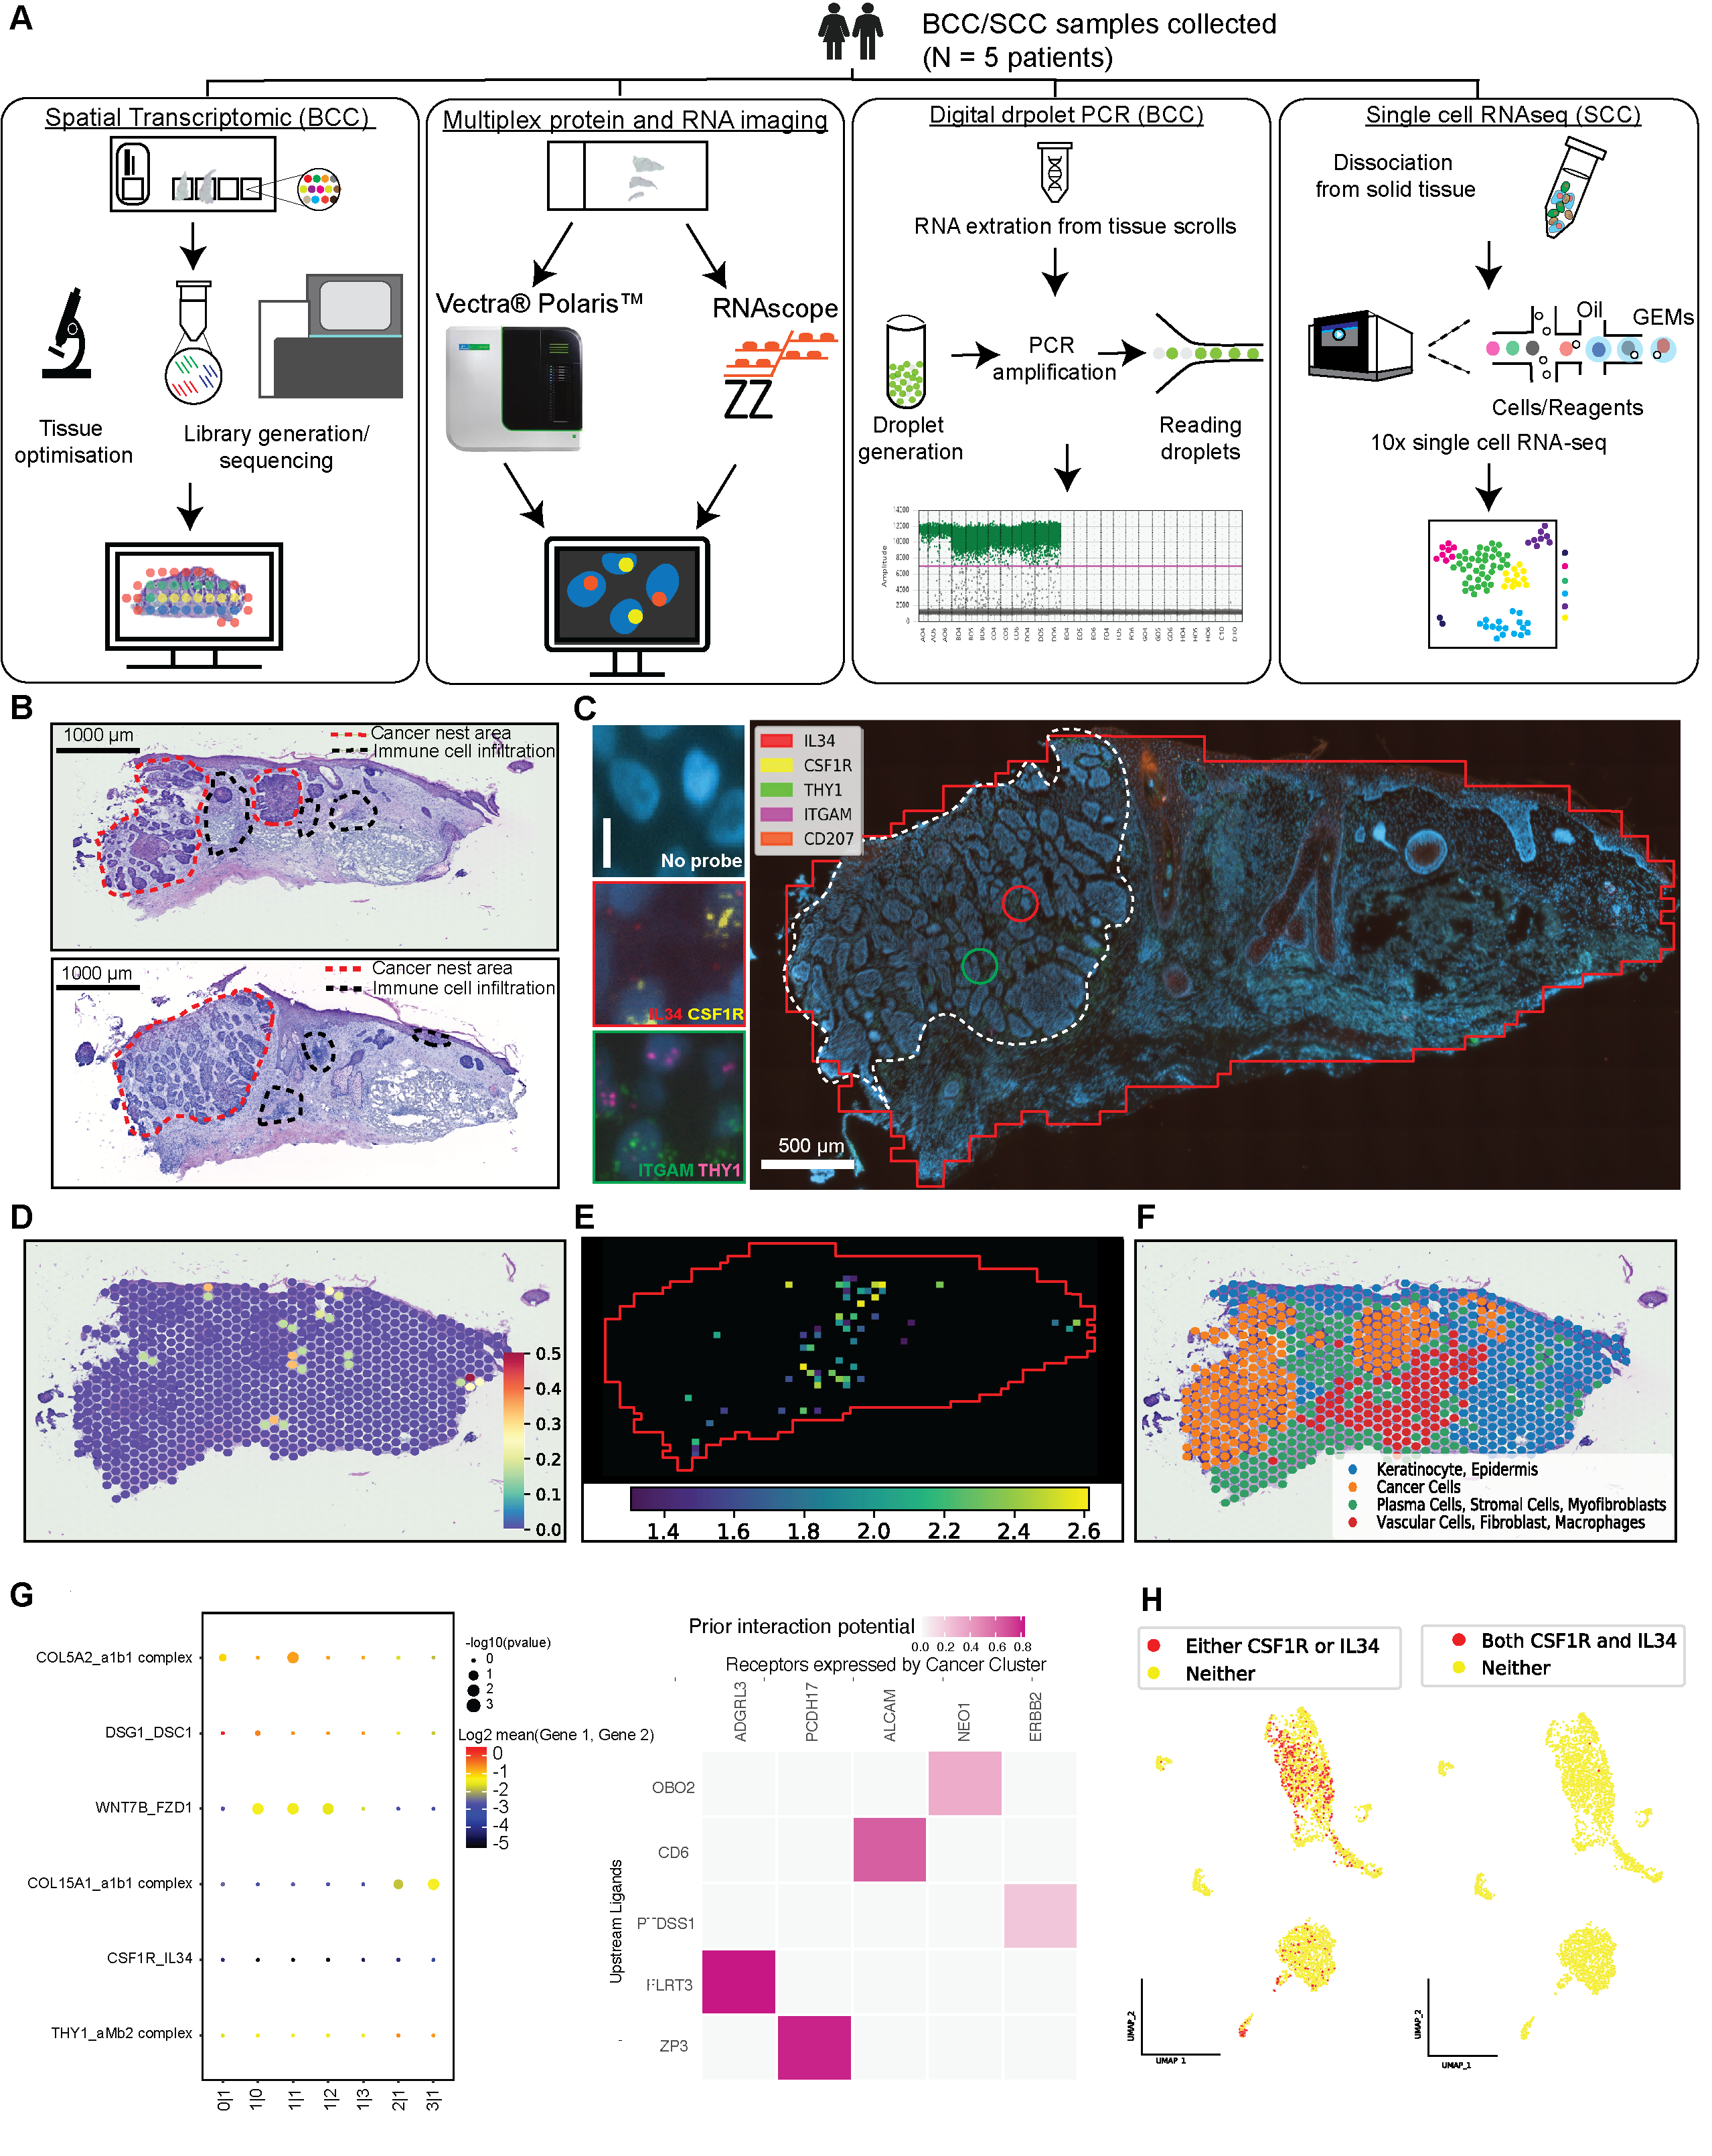
\includegraphics[width=\columnwidth]{Chapter2/Figures/Chapter2_Fig1_techsum.png}
    \caption{An integrated technological and computational approach to study cell-cell interaction across the whole tissue section. (A) A workflow illustrating the combination of four technologies to study L-R interaction in skin cancer tissue. (B) The annotated H\&E images of the two adjacent tissue sections that were used for Visium ST analysis (top) and the consecutive section of the same block used in RNAscope assay (bottom).(Legend continues on the following page.)}
    \label{fig:Chap2_figure1}
\end{figure}
\begin{figure}[t]
  \contcaption{(C) Target RNA molecule expression at a single cell level using RNAscope assay and the visualization of the local co-expression of two pairs L-R (D) Using ST-seq data and ligand-receptor expression analysis of neighbouring spots to determine significant local co-expression level of IL34-CSF1R(color bar showing the ligand-receptor score). (E) Results from our STRISH computational pipeline reported in this paper to analyse RNAscope imaging data, showing the detection of the local co-expression of IL34-CSF1R. The heatmap showing the windows with significant level of co-expression of ligand-receptor pair (scored by -log10 of p-values) (F) Spatial feature plots of the four distinct clusters defined by Louvain graph-based clustering. The annotation was based on differential gene and pathway analysis. The distribution of the cluster annotated as cancer was consistent with the location of cancer nests in the upper H\&E image shown in (B). (G) The inference of ligand-receptor based cellular communications from ST-seq data, using CellPhoneDB (left) and NicheNet (right). For CellPhoneDB prediction, top four highly active pairs of ligand-receptor and the two target pairs were selected for visualization . (H) The UMAP feature plots highlighted the cells that expressed either CSF1R or IL34 (red dots, left plot) and both CSF1R and IL34 (Cyan dots, right plot}% Continued caption
\end{figure}
% ***************************************************
\section{Detecting CCC from transcriptome-wide to targeted interaction}
\label{Sec:2.2_CCC_ST}	%CREATE YOUR OWN LABEL.
\subsection{Genome-wide analysis of ligand-receptor interaction using scRNA-seq}

We performed scRNA-seq analysis from the cells dissociated from three tissue samples (Table \ref{table:patientInfor}). scRNA-seq measures expression of all genes and data can be used for genome-wide prediction of cell-cell interaction (Figure \ref{fig:Chap2_figure1}A). Unsupervised clustering and differential expression analysis revealed 3 major subpopulations of epithelial (accounted for 80\% of total cell population) including Keratinocyte (KC) Basal, KC Differentiating (KC-Diff) and KC Cycling (Methods, Supplementary Figure \ref{fig:Chap2_Supfigure2}). Several immune and skin specific cell types were also identified including Lymphocyte, Myeloid, Dendritic, Melanocyte (Methods, Supplementary Figure \ref{fig:Chap2_Supfigure2}). To infer potential L-R pairs that are likely used as means of intercellular communication, we applied common single cell inference methods, CellPhoneDB \cite{efremova2020cellphonedb} and NicheNet pipeline \cite{browaeys2020nichenet} on our scRNA-seq dataset of matched samples, containing a squamous cell carcinoma sample tissue (SCC)  and a normal sample tissue from the same patient (Supplemental Figure S\ref{fig:Chap2_Supfigure2}A). NicheNet combines expression data with prior knowledge on gene signaling and gene regulatory networks to predict L-R pairs used by interacting cells (sender and receiver cells). We expected to use the detection of known IL34-CSF1R \cite{lin2008discovery} and THY1-ITGAM \cite{wetzel2004human} interaction to assess the sensitivity of the inference approach using scRNA-seq. The two pairs were not among the significantly detected pairs predicted by NicheNet (Supplementary Figure \ref{fig:Chap2_Supfigure2}A). To examine the relatedness of cells coexpressing the L-R pairs, we visualise L-R expression relative to cell cluster information in the UMAP space (Supplementary Figure \ref{fig:Chap2_Supfigure2}B-C). We found evidence of KC-Basal and KC-Diff cells that expressed IL34 while the receptor CSF1R was expressed by Myeloid and Lymphocyte (Supplementary Figure \ref{fig:Chap2_Supfigure2}C). However, THY1 and ITGAM were only expressed by a few cells with no distinct patterns of coexpression (Supplementary Figure \ref{fig:Chap2_Supfigure2}C). The results from examining THY1-ITGAM suggested the insensitivity of using scRNA-seq alone to study cell communication. Overall, we found that scRNA-seq can be utilized to study cell communication, but statistical test based on gene expression alone has low sensitivity and misdetects expected interactions.  

\subsection{Genome-wide analysis of ligand-receptor interaction using ST-seq}
We postulated that cell-cell communication could be more accurately assessed by using ST-seq, which preserves neighborhood information of interacting cells. We performed ST-seq on four tissue sections from four patients, with 2xSCC and 2xBCC tissue sections, (Table \ref{table:patientInfor}), (Figure \ref{fig:Chap2_figure1}B, \ref{fig:Chap2_figure1}D, \ref{fig:Chap2_figure1}F; Supplementary Figure \ref{fig:Chap2_Supfigure3}A, \ref{fig:Chap2_Supfigure4}A-C).  With ST-seq protocol, hematoxylin and eosin (H\&E) images allowed us to annotate cancer and immune cells, where the morphology revealed important tissue regions, including cancer nests, immune infiltrations and non-cancer regions (Figure \ref{fig:Chap2_figure1}B; Supplementary Figure \ref{fig:Chap2_Supfigure4}A-C). Additionally, adjacent tissue sections were used for RNAscope analysis as means of validation (Figure \ref{fig:Chap2_figure1}B, \ref{fig:Chap2_figure1}C; Supplementary Figure \ref{fig:Chap2_Supfigure5}).  From the same block, one section was used for ST-seq and another for RNAscope and comparing the ST-seq and RNAscope results for the two sections allows us to validate the ST-seq prediction data (Figure \ref{fig:Chap2_figure1}C-E; Supplementary Figure \ref{fig:Chap2_Supfigure3}, \ref{fig:Chap2_Supfigure4}), as discussed in the later section. 

With ST-seq approach, we reasoned that because each spot in the Visium slide contains a mixture of cells and these neighbouring cells (within a 55 $\mu$m diameter spot) can communicate if both ligand and receptor are detected in the spot (juxtacrine, autocrine, and short distance paracrine interactions). In addition, interaction between cells from two neighbouring spots (100 $\mu$m distance), through paracrine signalling, can likely occur if these spots display L-R co-expression. Therefore, local co-expression of L-R pairs within a spot or between neighboring spots in ST-seq data suggests possible cell-cell interaction. Based on the above assumptions, we implemented stLearn cell-cell interaction analysis to test for L-R local co-expression that was significantly higher than the background signal of random non-interacting gene-gene pairs. Using our stLearn software, we generated a cell-cell communication activity map across each of the whole tissue section for IL34-CSF1R from ST-seq data (Figure \ref{fig:Chap2_figure1}D; Supplementary Fig \ref{fig:Chap2_Supfigure3}A, \ref{fig:Chap2_Supfigure3}B; \ref{fig:Chap2_Supfigure4}4) \cite{pham2020stlearn}. Specifically, the heatmap of significant L-R interaction in the ST-seq data suggests the concentrated regions with high interaction within and surrounding the tumour areas as well as the immune infiltration regions. Independent pathological annotation also provided evidence for IL34-CSF1R interaction at the cancer-immune infiltration regions (Figure \ref{fig:Chap2_figure1}B; Supplementary Fig \ref{fig:Chap2_Supfigure3}A-C, \ref{fig:Chap2_Supfigure4}4). Additionally, unbiased clustering of gene expression using a graph-based approach in stLearn demarcates the tissue section into four distinct groups (Figure \ref{fig:Chap2_figure1}F). Based on differentially expressed genes and enriched pathways, we identified two major populations in cluster 1, observed in normal skin including keratinocyte (expressing CSTA, KRT6A) \cite{finnegan2019single}, epidermis (expressing KRT10, KRT14) \cite{ji2020multimodal}. Meanwhile the other three clusters expressed markers for cancer (SFRP5, GLI1) \cite{lacour2002carcinogenesis, ji2020multimodal}, stromal cells (CD40, THY1) \cite{koumas2003thy}, and macrophages (CXCL12, CD68). The distribution of the four cell types identified unbiasedly based on molecular profiles consistently overlapped with the pathological annotation based on the skin morphology and cancerous areas defined in H\&E images. These cell types support the ST-seq prediction of spatial locations where IL34-CSF1R interact (between inflammatory cells \cite{lin2019function}. The interaction activities were highest in the area with more cancer and immune infiltration cells, particularly in the epidermal compartment (Figure \ref{fig:Chap2_figure1}B; Supplementary Figure \ref{fig:Chap2_Supfigure3}E, \ref{fig:Chap2_Supfigure4}A-\ref{fig:Chap2_Supfigure4}B).  

\subsection{Comparisons of ligand-receptor interaction between ST-seq and scRNA-seq}
% ********* Enter your text below this line: ********
We found that computational methods that did not use spatial information failed to detect expected L-R interactions. From the CellPhoneDB analysis pipeline \cite{efremova2020cellphonedb}, a total 1024 possible combinations of L-R were tested using the ST-seq dataset. The dot-plot in Figure \ref{fig:Chap2_figure1}G demonstrated the low significance of the two L-R pairs, IL34-CSF1R and THY1-amb2 complex (ITGAM pathway) in comparison to the four other CellPhoneDB highest significance of the interaction pairs. We further applied NicheNet \cite{browaeys2020nichenet} workflow on the ST-seq data to integrate prior knowledge into the prediction. While NicheNet could identify interaction pairs that were directly linked to cancer (\ie CD6-ALCAM), the prediction also failed to detect the two pairs IL34-CSF1R and THY1-ITGAM. The expression plots of the four target markers overlayed to the tissue section (Supplementary Figure \ref{fig:Chap2_Supfigure3}C, \ref{fig:Chap2_Supfigure3}D) illustrated the low abundance across the tissue, which likely suffered from the inherent dropout (randomly misdetecting molecules due to the scRNA-seq protocol). The results suggest that for the noisy (high dropout) data and lowly-abundant genes, computational methods without spatial information like CellPhoneDB and NicheNet likely mis-identify meaningful cell-cell communication (Figure \ref{fig:Chap2_figure1}G, \ref{fig:Chap2_figure1}H). In contrast, the addition of spatial information to test for significant local-coexpression over the background, like stLearn, could detect such signalling events (Figure \ref{fig:Chap2_figure1}D; Supplementary Figure \ref{fig:Chap2_Supfigure3}E,  \ref{fig:Chap2_Supfigure4}A-\ref{fig:Chap2_Supfigure4}B). Although scRNA-seq and ST-seq enable us to test for thousands of ligand-receptor pairs, their inherent technical limitations in detection sensitivity necessitate the addition of independent validation experiments that are sensitive and are not sequencing based. Next, we describe RNAscope and our novel Spatial TRanscriptomic In Situ Hybridization (STRISH) pipeline as a powerful experimental method for validating cell-cell interaction within spatial tissue sections. 

% ***************************************************
\section{STRISH framework for detect cell co-localisation using FISH imaging}
\label{Sec:2.2_STRISH}	%CREATE YOUR OWN LABEL.

% ********* Enter your text below this line: ********
To overcome the limitations in detection sensitivity due to a lack of signal in the cancer region from the sequencing methods (scRNA-seq and ST-seq) and to achieve single cell resolution, we implemented RNAscope HiPlex assay. RNAscope HiPlex can detect upto 12 gene targets simultaneously at single-molecule sensitivity. In this study, we used whole tissue fluorescent microscopy images captured at 40x magnification to determine RNA interaction at cellular resolution. Three different fluorophores (Cy3, Cy5 and Cy7) were used in two iterative wash-stain rounds to label the five distinct target genes, including THY1, IL34, and CSF1R, CD207 and ITGAM (Figure \ref{fig:Chap2_figure1}C). The zoom-in images from a cancer nest area (marked as a white dashed line, and two red/green circles - IL34 and CSF1R in a red box and THY1 and ITGAM in a green box) show distinct coexpression of neighbouring cells at single-cell resolution, suggesting cell to cell interaction for each of pair compared to no signal in the 'Negative' control. 

To automate and improve the accuracy of detecting L-R interaction across the whole tissue section based on fluorescent data, like RNAscope, we developed a computational pipeline STRISH. STRISH pipeline consists of two phases, starting with a cell local co-expression detection step to define spatial neighbourhood, followed by scoring, statistical testing and visualizing significant local co-expression (Figure \ref{fig:Chap2_figure2}A; Method Algorithms 1,2). Local co-expression is defined as the expression within a tissue area containing fewer than a threshold number of cells (depending on tissue types), for example fewer than 100 cells. The pipeline runs a series of positive-cell detection iterations to find regions that contain lower than the predefined threshold of neighboring cells and subsequently determines the number of L-R co-expression within these regions (refer to the Method section about STRISH algorithm). The L-R co-expression scores are then used for statistical test of significant coexpression over the null distribution of random, non-interacting gene-gene pairs. Across the tissue samples, we observed considerable interaction of IL34-CSF1R around the areas where the cancer nests are in both BCC and SCC, particularly in the epidermal compartments (Figure \ref{fig:Chap2_figure1}E, 2B). Interestingly, compared to RNAscope data we observed a similar pattern in ST-seq data, with many spots that were predicted to have cell-cell communication through IL34-CSF1R located in cancer and epidermis regions.  

We further assessed the performance of STRISH by measuring the interaction of another less abundant L-R pair, THY1-ITGAM. We found lower signal and less wide-spread interaction of THY1-ITGAM that were localized to the dermal compartments (Figure \ref{fig:Chap2_figure2}B). By comparing the number of the tissue regions (through STRISH windows) where local co-expression was found, we noticed the average count of the windows with THY1 and ITGAM co-expression was, on average, 2.5 times less than those of IL34-CSF1R. Similarly, the normalized local co-expression in the same STRISH windows for ITGAM were also lower than that of IL34. We noted that most of the STRISH-detected local co-expression of THY1 and ITGAM were clustered densely around the adjacent areas of the immune cell infiltration. At the core, STRISH is constructed based on a new data structure called STRISH\_Object which encapsulates the data structure from AnnData \cite{wolf2018scanpy}. Thus, STRISH is highly compatible with other single-cell based platforms (\ie Scanpy \cite{wolf2018scanpy} and Squidpy \cite{palla2022squidpy}). STRISH can also accommodate the visualization of expression level of each marker at single-cell for quality inspection and facilitate the external validation/correlation of cell positive with markers of interest (i.e ddPCR) (Figure \ref{fig:Chap2_figure2}C). We also found that STRISH was quantitative and provided the capability of counting interaction events, an important utility that is needed in the cellular communication research (Figure \ref{fig:Chap2_figure2}D; Equation \ref{chap2:eq:02} ,\ref{chap2:eq:03}). Overall, we found that RNAscope data analysed by STRISH could detect cell-cell communications at a higher sensitivity than ST-seq and scRNA-seq. 
\begin{figure}[htp]
    \centering
    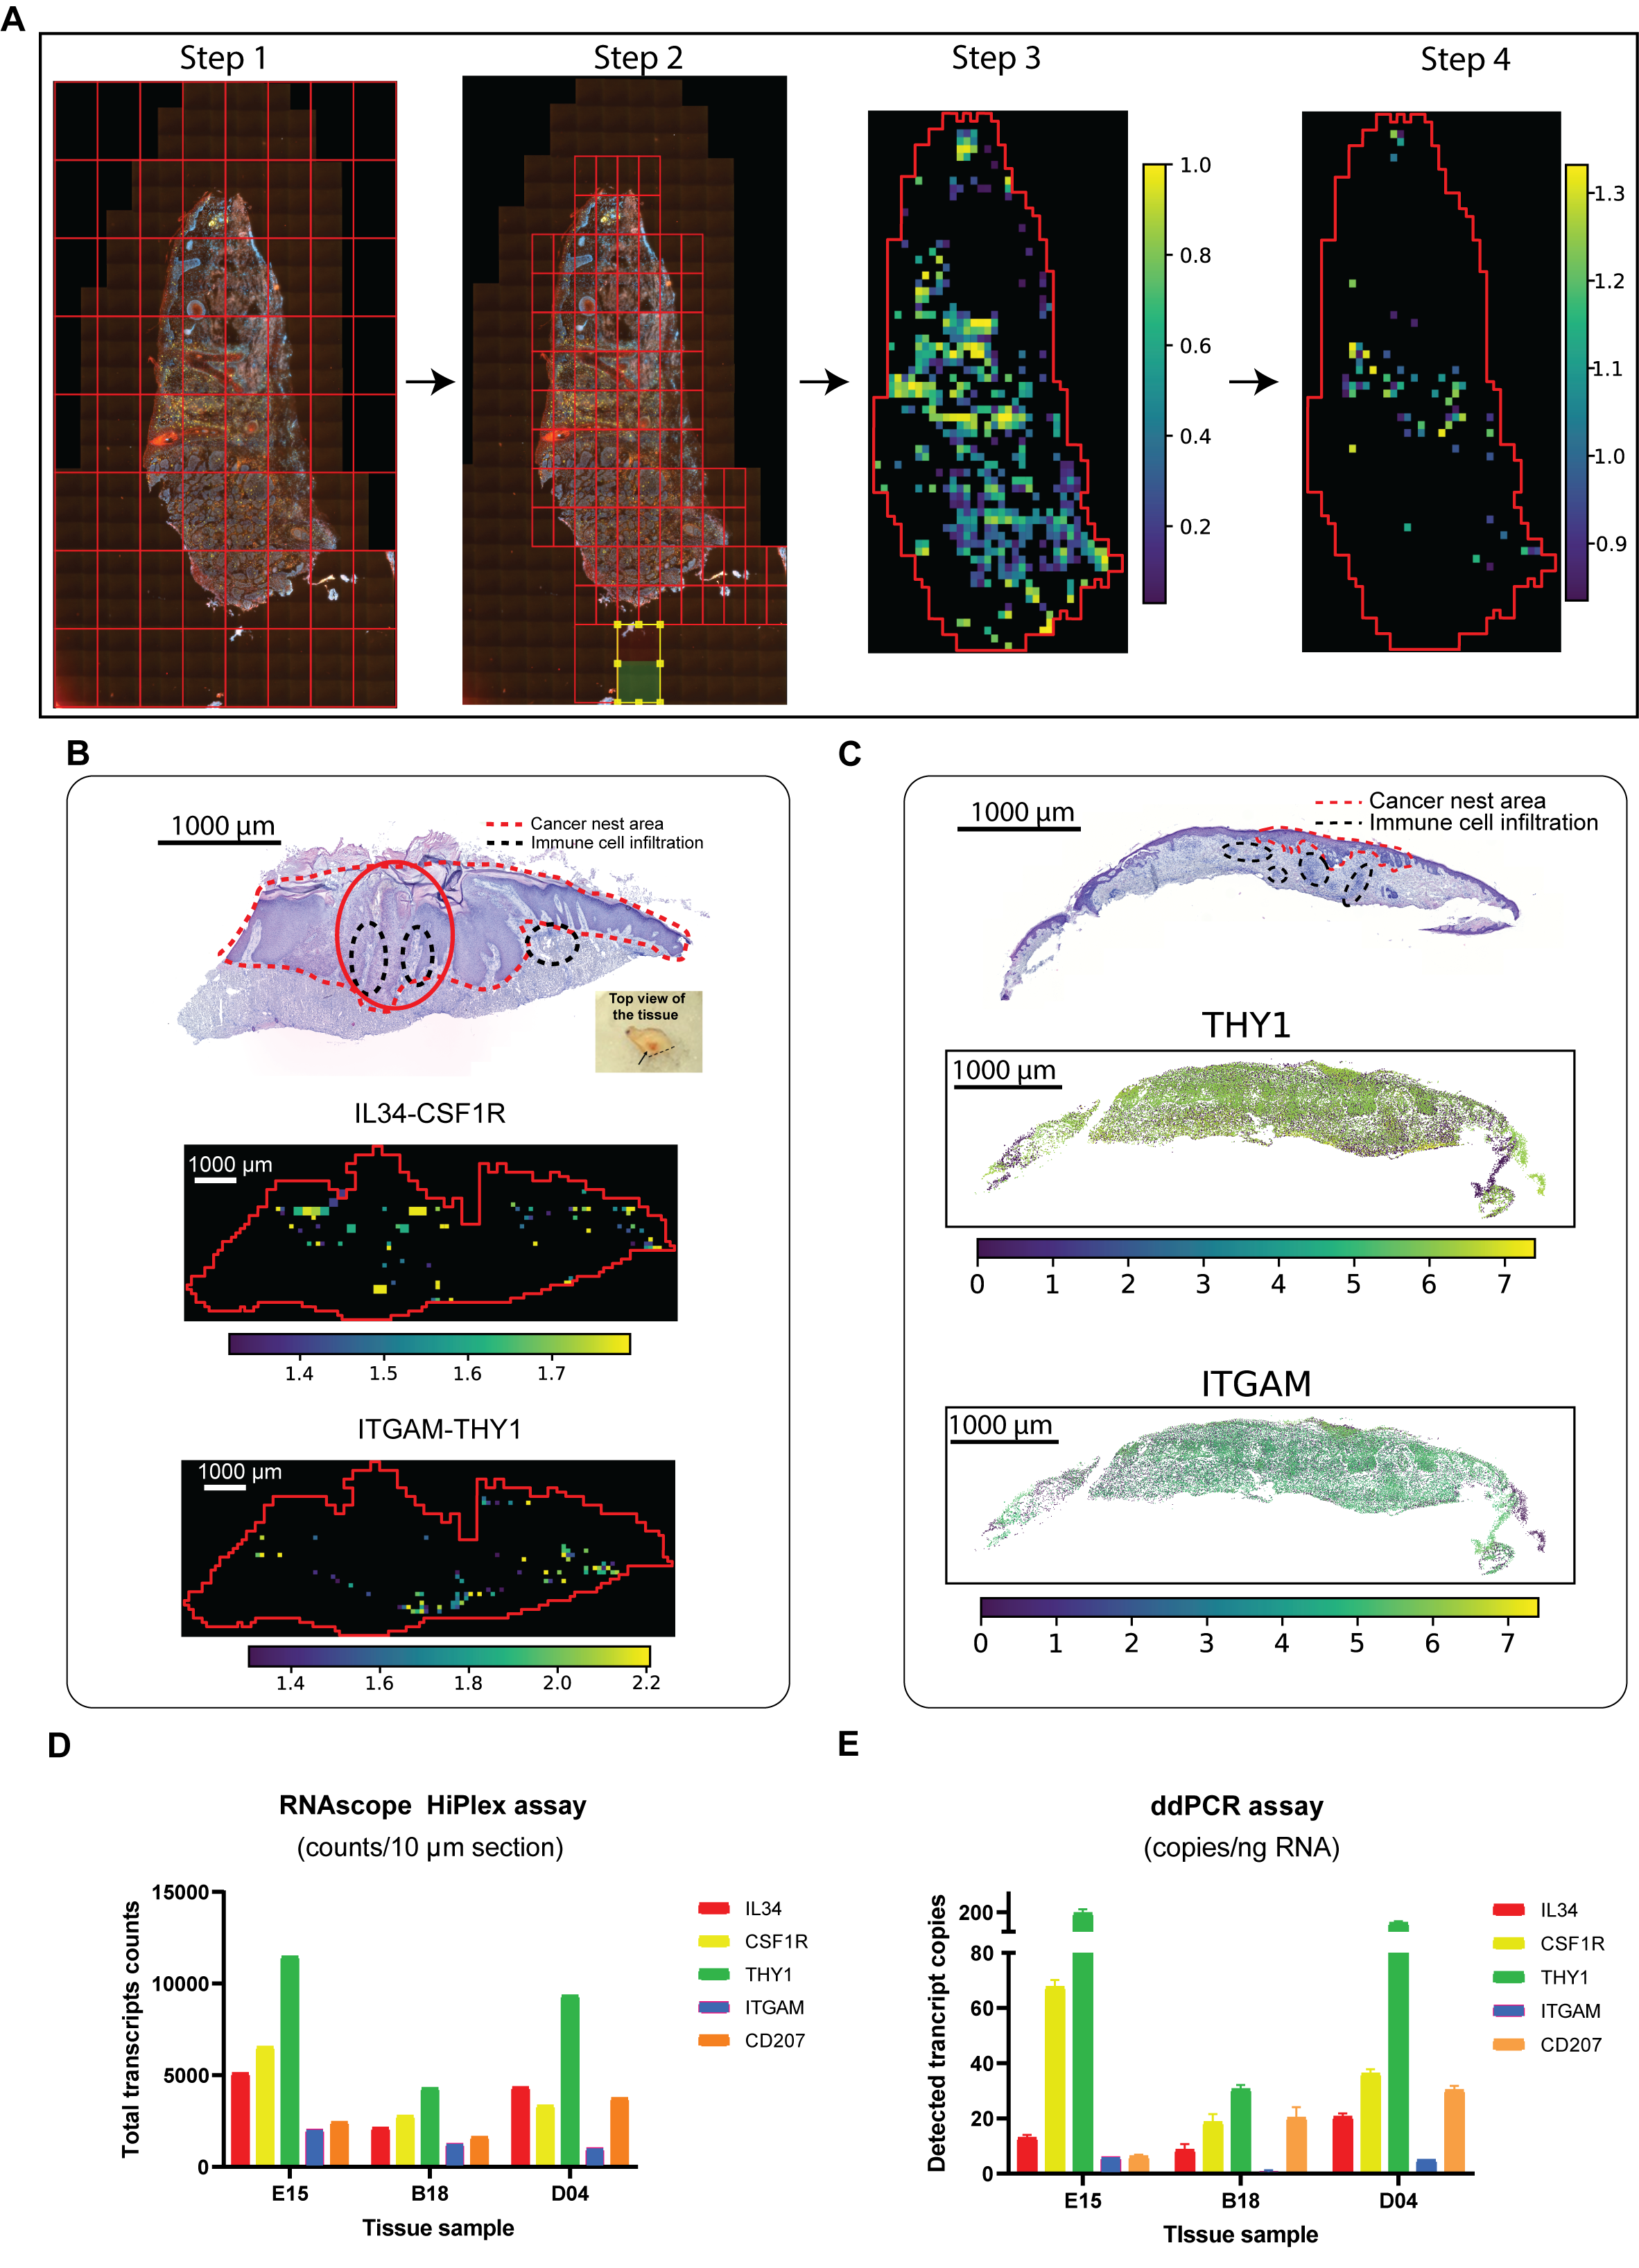
\includegraphics[width=0.95\columnwidth]{Chapter2/Figures/Chapter2_Fig2.png}
    \caption{Detection of target RNAs in skin cancer patients by collective transcriptomic and genomic methods. (A) STRISH analysis method to scan for local-coexpression of ligan-receptor pairs. Steps from raw RNAscope data to creating a tissue-scale heatmap (significant activity map) of local co-expression of target mRNAs are shown. (Legend continues on the following page.) }
    \label{fig:Chap2_figure2}
\end{figure}
\begin{figure}[t]
  \contcaption{Brifely, STRISH splits the image into large, even-size windows (Step 1). Based on cell segmentation and the count of number of cells per window, STRISH further splits a window into smaller ones if the window has more cells than required and discards those windows without cells (Step 2). Using the remaining windows which contains cells expressing L-R, STRISH can perform the co-localization scoring and statistical test to produce a heatmap of the most significant windows in spatial context (Step 3 and 4). (B) From top to bottom: annotated H\&E of SCC patient ID-F21 and the corresponding heatmaps (activity maps) of local co-expression for the two L-R pairs, IL34-CSF1R and THY1-ITGAM, respectively. (C) The expression levels of THY1 and ITGAM using RNAscope signal measurement within the cells throughout the tissue of the patient ID-D04. (D) and (E) The absolute copy number of the target mRNAs counted using ddPCR and RNAscope assays.}% Continued caption
\end{figure}
\subsection{Highly sensitive detection of ligand and receptor expression by ddPCR}
While RNAscope is expected to be able to detect single molecules in each cell, scanning through a whole tissue section with millions of cells may lead to noise and reduced accuracy due to tissue heterogeneity. ddPCR, on the other hand, enables to sensitively detect and quantify single molecules from tissues, albeit spatial information is absent. To further confirm the presence of ligand and receptor in the tissue, we performed ddPCR on the same cancer tissue block (Supplementary Figure  \ref{fig:Chap2_Supfigure6}). The transcript copy number per input RNA of each gene was presented in a bar plot (Supplementary Figure \ref{fig:Chap2_Supfigure2}E). ddPCR signal was highly consistent between cells (droplets) and both L-R pairs were detected. Strikingly, the result from ddPCR was highly consistent to that of RNAscope data (Figure \ref{fig:Chap2_figure2}D, \ref{fig:Chap2_figure2}E), with Pearson correlations at 0.95, 0.89 and 0.94 for the patient samples tested, ID-E15, B18 and D04, respectively. The ddPCR results support the quantitativeness of using RNAscope for measuring target gene expression, suggesting the suitability of using RNAscope for detecting and quantifying cell-cell interaction. 

\subsection{Extending the application of STRISH to analysing protein fluorescence data to detect L-R interaction}
While scRNA-seq, ST-seq and RNAscope data can be used for inferring cell-cell interaction, they measure RNA and thus not directly reflecting the interaction at protein level. We generated multiplex protein immunofluorescence data for a SCC cancer sample using multispectral imaging with primary antibodies-Opal pairing technologies (Akoya biosciences). On the same tissue section, six cancer and immune markers were detected simultaneously, including a L-R pair (PD-1 and PD-L1), PanCK (epithelial cancer marker), CD8 (T cell marker), CD68 (Macrophage marker), FoxP3 (T regulatory cell marker), (Figure \ref{fig:Chap2_figure3}A). 

Our STRISH pipeline can be flexibly applied to protein data. Here, we implemented the STRISH pipeline to detect the local expression levels of the L-R pair PD-1 and PD-L1, well known signalling molecules used in immune and cancer cell interaction \cite{pardoll2012blockade}, (Figure \ref{fig:Chap2_figure3}B). We divided the fluorescent tissue image into multiple smaller areas containing fewer than 100 cells, defined as a local neighbourhood region (refer to Algorithm \ref{Chap2:Alg:01}, \ref{Chap2:Alg:02} and Method Section). We then quantified the cell expression on the window for either PD-1 or PD-L1 (refer to Algorithm \ref{Chap2:Alg:02}, Method Section). The activity map of PD-1 and PD-L1 interaction is shown as a tissue heatmap with colors representing the normalised count (normalisation of all cells within each window) of PD-1 and PD-L1. The automated STRISH detected regions with high co-expression of PD-1 and PD-L1 were visually examined, separately for each of the two channels, PD-1 and PD-L1 (Figure \ref{fig:Chap2_figure3}C). Similar to the RNAscope data, we showed that STRISH could detect PD-1 and PD-L1 local co-expression accurately. Visual inspection of positive and negative windows (Figure \ref{fig:Chap2_figure3}C) shows the unique new feature of STRISH in that it detects local co-expressing cells of the L-R pairs, in contrast to other methods that only detect the co-expression of two or more proteins from the same cell. 
\begin{figure}[htp]
    \centering
    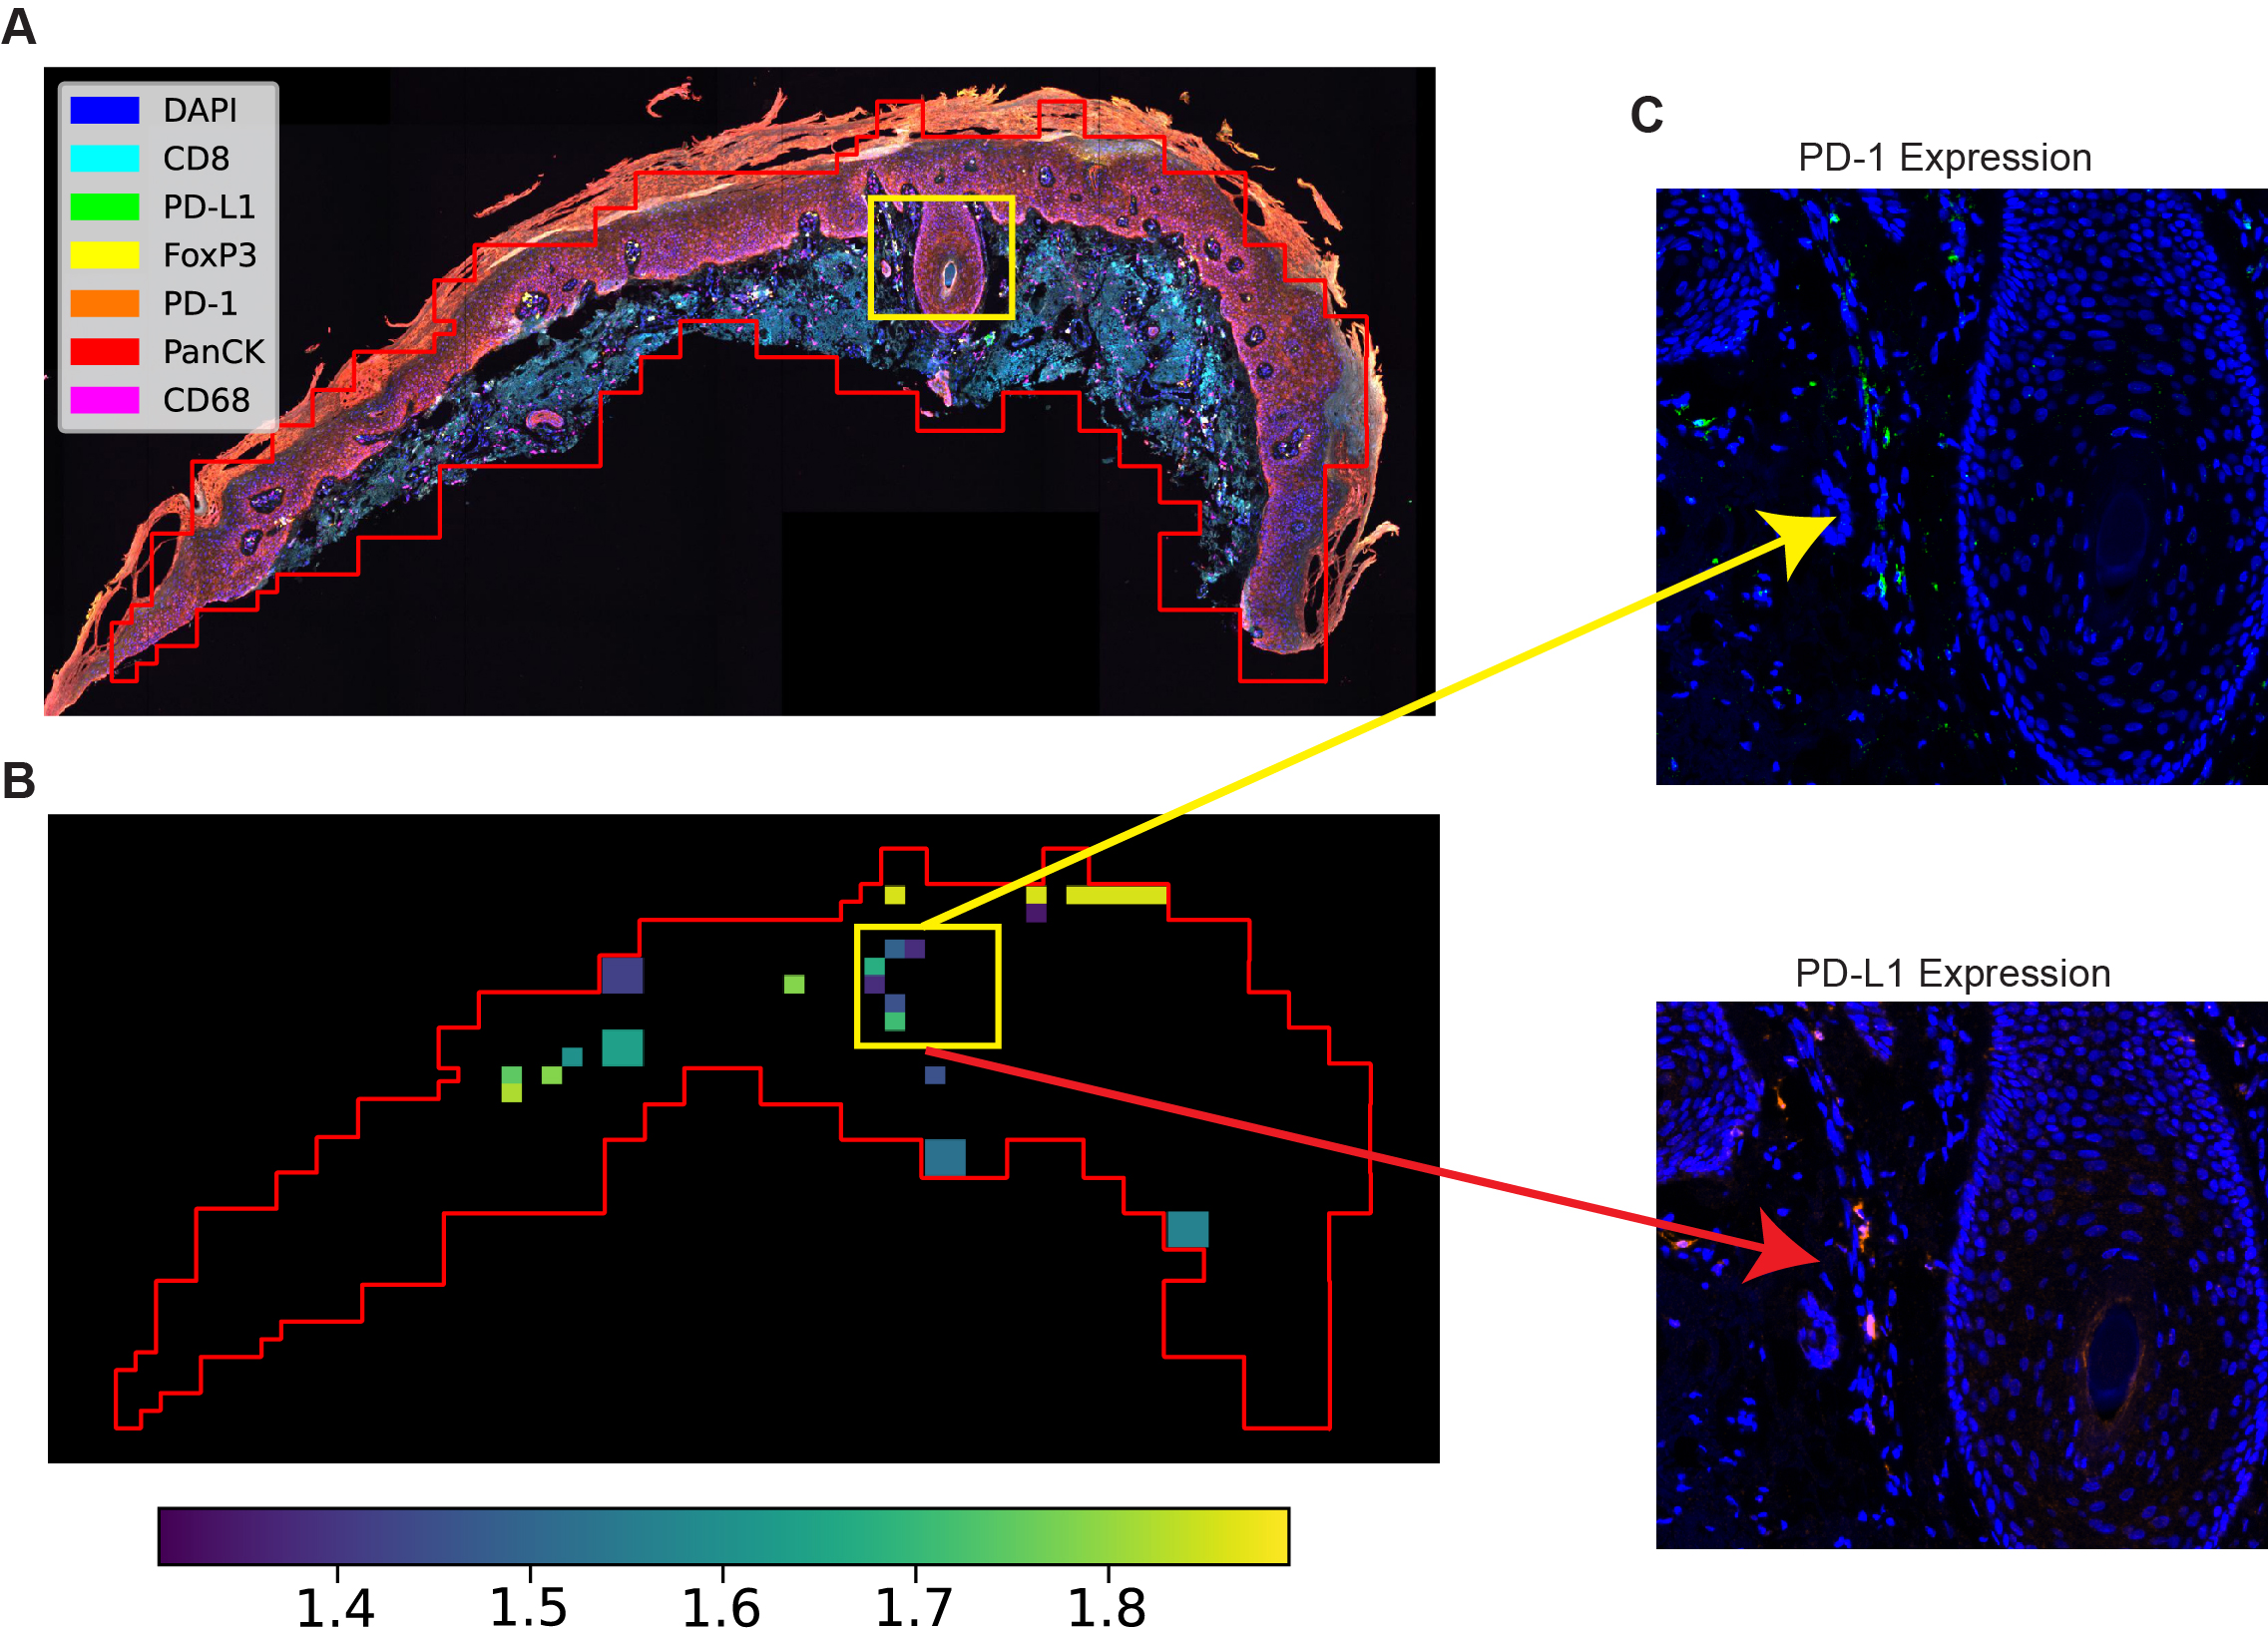
\includegraphics[width=0.8\columnwidth]{Chapter2/Figures/Chapter2_Fig3.jpg}
    \caption{ STRISH application to protein data. (A) A multispectral image captured using MOTiF™ PD-1/PD-L1 panel (6 proteins and a DAPI) of an SCC cancer tissue section. (B) STRISH significant test heatmap (activity map) suggesting the tissue locations with high (yellow color) or low (dark color) level of protein local co-expression after the statistical test for the ligand-receptor pair PD-1 and PD-L1 (the value shows in color bar indicate negative log p-values). The tissue contour was plotted using the windows of neighboring cells identified by STRISH. (C) A close-up visualization of the areas identified as the existing cells local co-expression of PD-1 and PD-L1 by STRISH.}
    \label{fig:Chap2_figure3}
\end{figure}
% ***************************************************
\section{Methods and quantitative validation}
\label{Sec:2.3_validation}	%CREATE YOUR OWN LABEL.
\subsection{Single cell RNA sequencing data analysis}
All three gene-barcode count matrices were loaded and merged into a single SeuratObject using Seurat/4.0.0 in R/4.0. We removed cells with fewer than 200 or more than 5000 genes and cells with over 20\% of all reads mapped to mitochondrial genes. Seurat canonical correlation analysis was performed to correct batch effect and integrate the samples. The processed expression matrix was scaled to 10,000 reads/cell, normalized and only the top 5000 most variable genes were kept for PCA dimensionality reduction. The top 50 PCs were used to generate UMAP plot and clustering the cells using Louvain graph-based in Seurat (Supplementary Figure S \ref{fig:Chap2_Supfigure2}B). Using FindClustering function with the resolution of 0.7, we determined 12 subpopulation of cell types. Differential expression (DE) was performed to find top 100 differentially expressed genes for each cluster. Clusters with similar top DE genes were combined, which subsequently resulted in 3 different Keratinocytes subtypes including KC Basal (KRT15, KRT14, CXCL14  upregulated), KC Differentiating (KRT1, 2 and 10), KC Cycle (TOP2A, STMN1)  \cite{joost2016single, ji2020multimodal} and 2 skin specific cell types Melanocyte (DCT, TYR, TYRP1), Pilosebaceous (DEFB1, DEFB2) \cite{belote2021human}. Besides, we identified three immune cell types that commonly found in skin tissue  Lymphocyte (CD8, CD4), Myeloid (highly expressed CD207, S100A9 and HLA-DRA), Plasma Dendritic cells (CD20, CD79 upregulated) \cite{ji2020multimodal}.          

To infer cell-cell interaction through L-R pair, we applied NicheNet L-R prediction pipeline \cite{browaeys2020nichenet} on our two scRNA-seq datasets of cancer and normal samples from a patient (Table \ref{table:patientInfor}). We ran the gene differential expression analysis for two conditions of cancer and normal. For the deferentially expressed genes we used top 12 upstream ligands, then filtered the prebuilt ligand receptor network to find the corresponding upstream receptor and plotted the heatmap of potential interaction in Supplementary Figure \ref{fig:Chap2_Supfigure2}A.
\subsection{Visium spatial transcriptomics sequencing and analysis}
The Visium raw sequencing data in BCL format was converted to 110,782,035 FASTQ reads using bcl2fastq/2.17. The reads were trimmed by cutadapt/1.8.3 to remove sequences from poly-A tails and template-switching-oligos. We used SpaceRanger V1.0 to map FASTQ reads to the cellRanger human reference genome and gene annotation for GRCh38-3.0.0. On average, for each spot we mapped 94,710 reads and detected 1,428 genes. The count matrix of the Visium data was preprocessed to remove genes that expressed in less than three cells, followed by the normalization, log transformation and scaling. For spot clustering, we first performed gene expression normalization using spatial morphological information from the H\&E image then clustered the spots using Louvain community detection algorithm. The normalization was to reduce the technical limitation in detecting lowly expressed genes. Besides, a neighborhood graph of spots was built based on the reduced dimensional space, followed by the application of Louvain community detection to group similar spots into clusters. 

We performed ST-seq on four tissue sections from three BCC/SCC patients (patient ID-E15, B18, F21). The prediction of cell-cell interaction of a pair IL34 and CSF1R analysis is produced by the stLearn package (Pham et al.) (Figure \ref{fig:Chap2_figure1}C, Supplementary Figure \ref{fig:Chap2_Supfigure3} , \ref{fig:Chap2_Supfigure4}).  For L-R prediction with CellPhoneDB, we applied the default parameters \cite{browaeys2020nichenet, efremova2020cellphonedb}  and used a curated database v2.0.0. Similar to scRNA-seq analysis for cell-cell communication via L-R pairs, we applied NicheNet L-R prediction on ST-seq data. The upstream ligands were ranked by descending Pearson values and top 5 ligands were pulled out to sort out the corresponding upstream receptors (Figure \ref{fig:Chap2_figure1}G). 

\subsection{Multiplexed RNA in-situ hybridization with RNAscope}
The following target probes to detect L-R interaction were designed by ACD probe design Team and used for the RNAscope HiPlex assay (ACD Cat. No. 324110): THY1 (ADV430611T2), IL34 (ADV313011T3), CSF1R (ADV310811T4), CD207 (ADV809521T7), and ITGAM (ADV555091T8). The slide was stained with a mixture of the 5 probes to allow them to hybridize with RNAs. The negative control slide was stained with RNAscope HiPlex 12 Negative control Probe that was provided in the kit. The images were captured by Axio Z1 slide scanner (Zeiss) with an appropriate adjustment of each fluorescent intensity. The first round of images was performed using 4 filters including DAPI for nuclei, Cy3 for THY1, Cy5 for IL34, and Cy7 for CSF1R. For the high resolution of an image, a 40x objective was used and the Z-stack interval was set up to 1.5µm resulting in 9 of Z-slices for each slide. The images were further processed by ZEN software (version 3.2) for manual stitching and adjusting contrast/brightness.

\subsection{STRISH pipeline for cell-cell interaction analysis}
To uncover the interaction of immune cells and cancerous cells in the whole BCC/SCC tissue section, we developed an analysis pipeline, called STRISH. A standard multiplexing RNAscope which captured the cell nuclei and RNA fluorescence signal in a multidimensional image format is used the input for the pipeline. First, we utilised stardist \cite{schmidt2018cell} model and QuPath software \cite{bankhead2017qupath} to perform cell detection. We applied the preprocessing step to calculate the mean signal values of all 9 of Z-slices following Equation (1), which aggregate the signal form multiple Z slices into one layer. Noted that during the RNAscope imaging, the slide was scanned using Z-stack interval which resulted in multiple slices image. It is possible to carry out cell detection at every Z-slice image. However, stardist has consistently outperformed other models in detecting overlapped signal from nucleus \cite{schmidt2018cell}. Thus, it allows accurately capturing the cell with single layer image and avoid computational inefficient. The cell detection process transforms every cell from DAPI channel in image into a polygonal object (a margin for cell membrane is added to nuclei boundary). Secondly, the mean intensity of RNA fluorescence signal within cell boundary was measured and assigned to the corresponding cell (Figure \ref{fig:Chap2_figure2}A Step 1). After that, STRISH provides a function converts into single cell object called STRISH\_Obj which customised from AnnData \cite{wolf2018scanpy}. 
\begin{equation}
c_{i} = \frac{\sum_{j=1}^{n_{slides}}(c_{ij})}{n_{slides}}
\label{chap2:eq:01}
\end{equation}
where $c_i$ indicates the DAPI or RNA marker channel, $j$ is an iterator of the Z-slices.

Finally, several data prepressing functions are available within STRISH to remove the effect of artificially high background from fluorescent intensity (outlier) and cells that are too large or small (false detection), By default, STRISH clips that cell’s marker expressions to 95th percentile of all intensities and remove cells that are too small (less than 5th percentile of all areas). To determine more specific thresholds, STRISH enables several functions for quality control and plotting the marker expression of every cell (\ie Fig \ref{fig:Chap2_figure2}C).

To quantitatively measure the local co-expression of each window, we defined a scoring function to score the number of cells that express either ligand or receptor in the same window following the Equation (2). Coexpression score considers the frequency of the cell that express the ligand and receptor reside in each window. Besides, the coexpression score is constrained to the presence of both marker ligand and receptor in the same window which increase the likelihood of interaction between cells through that pair of L-R (Figure \ref{fig:Chap2_figure2}A Step 3). Once every window is scored, a statistical test for the most significant windows is used.     

The downstream analysis for detecting cell local co-expression by window scanning in STRISH is summarised in Algorithm \ref{Chap2:Alg:01}. More specifically, the STRISH functionality for cell local co-expression was developed to iteratively scan through the image, using a neighbourhood window detection strategy to find the target regions with cells expressing the marker of interest. First, a cell scanning windows process is initiated to cover a broad area of scanning with dimensions for width and height set to a predefined rate of the whole scan images. While iterating through the stack of all the existing windows, STRISH will discard those windows with fewer than two cells (cell count is based on DAPI signal). For each window, where the number of detected cells is greater than a threshold (user’s defined threshold depending on cancer tissue types), STRISH further splits it into smaller windows (the default rate is 50\% of the current considering window dimension) and adds these smaller windows into the iteration stack (Figure \ref{fig:Chap2_figure2}A Step 2). Finally, windows that pass the cell threshold check are subjected to the next step to detect co-expression. Using expression level of each marker for every cell as the features, STRISH performs cell classification through standard single-cell cell clustering (\ie Leiden clustering from scanpy \cite{wolf2018scanpy}) and/or signal gating on respective marker signal.
\makebox[\linewidth]{%
\begin{minipage}{\dimexpr\linewidth}
\begin{algorithm}[H]
\SetAlgoLined
\SetKwInOut{Input}{input}
\SetKwInOut{Output}{output}
\Input{$cell\_segmentation\_file$ \CommentSty{\#cell segmentation and biomarker signal measurement result}, \newline 
$scan\_image\_fn$ \CommentSty{\#microscopy image for analysis}, \newline
$threshold$ \CommentSty{\#theshold for cell count per window} }
\Output{$cell\_colocalised$  \CommentSty{\#dataframe of cells colocalised by target ligand receptor pair}}
	$cell\_segment\_data = read\_cell\_detection(cell\_segmentation\_file)$\;
	$scan\_img\_data = read\_img(scan\_image\_fn)$\;
	$init\_windows = add\_window\_to\_image(scan\_img\_data.shape)$\;
	$cell\_count = window\_cell\_detect(init\_windows, cell\_segment\_data)$\;
	\While{$init\_windows.count() > 0$ or $count\_cell > threshold$ }{
	$windows\_available = get\_all\_windows()$\;
	\For{$window~\in~windows\_available$}{
	$count\_cells = window\_cell\_detection(dapi\_channel, window)$\;
	\uIf{$count\_cells \leq 2$}{
	    \CommentSty{\#Remove the windows with less than 2 cells as there is no possible multiple cells interaction}\\
	$windows\_available.remove\_window(window)$\; 
	\uElseIf{$count\_cells >2$ and $count\_cells \leq threshold$}{
        \CommentSty{\#Run cell detection with respect to other marker channels}\\
        $cells\_express\_ligand = run\_cell\_detection(ligand\_channel)$\;
    	$cells\_express\_receptor = run\_cell\_detection(receptor\_channel)$\;
    	$return\_to\_file(count\_cells, cells\_express\_ligand, cells\_express\_receptor)$\;
    	$windows\_available.remove\_window(window)$\;
    }
    \Else{
        \CommentSty{\#Number of cells in current window greater than the threshold, split the window into smaller windows}\\
        $new\_windows = add\_annot\_windows(widow\, subset_rate)$\;
   \CommentSty{\#Remove the current window as the new subset windows are spawned from and replaced the current window }
        $windows\_available.remove\_window(window)$ \;
    }
	}
	}
	}

 \caption{Cell detection by window scanning throughout the tissue section}
 \label{Chap2:Alg:01}
\end{algorithm}
\end{minipage}
}
To quantitatively measure the local co-expression of each window, we defined a scoring function to score the number of cells that express either ligand or receptor in the same window following the Equation \ref{chap2:eq:02}. Coexpression score considers the frequency of the cell that express the ligand and receptor reside in each window. Besides, the coexpression score is constrained to the presence of both marker ligand and receptor in the same window which increase the likelihood of interaction between cells through that pair of L-R (Figure \ref{fig:Chap2_figure2}A Step 3). Once every window is scored, a statistical test for the most significant windows is used.
\begin{equation}
    coexpression\_sc_{wi} = \begin{cases}
    \frac{n_{cell\_ligand_{wi}} + n_{cell\_receptor_{wi}} }{n_{total\_cell_{wi}}}&;\text{if $ n_{cell\_ligand_{wi}} \neq 0$ and $n_{cell\_receptor_{wi}} \neq 0$}\\
    0              & ;\text{if $ n_{cell\_ligand_{wi}} = 0$ or $n_{cell\_receptor_{wi}} = 0$}
    \label{chap2:eq:02}
\end{cases}
\end{equation}

\subsection{Test of significance windows with L-R colocalization}
To validate test for the significant of the cell-cell interactions based on colocalization scored among all the positive windows, STRISH performs the a statistical test to compare the level of co-localisation of the pair of L-R of interest with the random combination of two pair of markers available for the same window and across all the positive windows. Briefly In summary, STRISH finds tissue locations (windows) that have coexpression of L-R pairs higher than random expression in other windows and by other non L-R pairs. There are two randomization procedures, testing for the expression level relative to random non L-R pair at one location (one window), and testing for significant expression of one of co-localisation of L-R pair relative to all locations a window (equation \ref{chap2:eq:03}). Firstly, the means of cells co-localisation for both ligand or receptor within every window $w_i \neq 0$ is compared to the random combination of two a positive to ligand and a target non-receptor marker from the same window. The comparison between real pair of L-R cell co-localisation with the matched randomized pairs allows us to show test for if there are significantly more the abundant presence of the cells expressing  the ligand and receptor within a window than cells co-expressing random non L-R pairs. Secondly, for all the windows that have the positive mean of co-localisation score of the same L-R, we tested if certain windows had  are tested against each other to identify for the significant more cells co-expressing the pair than the remaining  most significant windows across the tissue. This test reduces false positive detection, because while the scanning windows approach could capture the region of colocalisation of cells expressing the ligand and receptor, the colocalisation can be random expression of the pairs that happened to be in the same window, but was at a low level of cells can also be at random. The second randomness test aims to identify the windows which have the highest frequency of colocalisation of the target L-R compared with all other windows throughout the tissue. The combination of two statistical test generates will provide a P value for each window which correspond to either significant or insignificant colocalisation.

\begin{equation}
    P_{wi} = \frac{\sum_{i=1}^{m}(coexpres\_sc_{wi} > coexpres\_sc_{random\_pairs_{wi}})+ \sum_{j=1}^{n-1}(coexpres\_sc_{wi} > coexpres\_sc_{pos\_lr_j}) }{total\_random_{random\_pairs} + total\_window_{pos\_lr}}
    \label{chap2:eq:03}
\end{equation}

Where,	$coexpres\_sc_{wi}$  is colocalisation score of each window $w_i$, calculated as in Equation \ref{chap2:eq:02}, ($m$ is the number of windows in the dataset); $coexpres\_sc_{random\_pairs_w}$ is the colocalisation score of the same window $w_i$, calculated for random pairs of other markers in the dataset that are known to not interact, as calculated in Equation \ref{chap2:eq:02}; the number of random pairs is the permutation of $\frac{(n*(n-1))}{2}$ (where n is the number of markers in the dataset); $coexpres
\_sc_{pos\_lr_j}$is the colocalisation scores of all the windows within the tissue that express the same ligand and receptor pair as in $w_i$; $total\_random_{random\_pairs}$ denotes the total number of windows with randomized pairs of markers; $total\_window_{pos\_lr}$  denotes the number of windows with the same pair of target ligand-receptor

We developed a Python-based pipeline to construct the heatmap of cell local co-expression. 
As there were two rounds of RNAscope imaging, we added to STRISH an image registration functionality. For the interaction of ITGAM and THY1, as the signal of the genes were captured in two separated imaging rounds with the respective stitching in post process, some variants were introduced (Supplemental Figure S\ref{fig:Chap2_Supfigure7} A-B). To overcome the unaligned tissue layout, we performed image registration to map one image to the other (Supplemental Figure S7C). The image registration is performed solely using SITK library \cite{lowekamp2013design, yaniv2018simpleitk}.  

\makebox[\linewidth]{%
\begin{minipage}{\dimexpr\linewidth}
\begin{algorithm}[H]
\SetAlgoLined
\SetKwInOut{Input}{input}
\SetKwInOut{Output}{output}
\Input{$target\_lr$ \CommentSty{\#pair of target ligand receptor}, \newline 
$random\_pair\_markers$ \CommentSty{\#random pair of ligand receptor}, \newline
$windows\_available$ \CommentSty{\#list of windows with cell colocalisation }, \newline
$p\_threshold $ \CommentSty{\#threshold for statistical significant testing}}
\Output{$sig\_windows$  \CommentSty{\#list of windows with significant level of lr colocalisation}}
	$target\_lr, random\_pair\_markers, window\_available, p\_threshold = input()$\;
    $coexpres\_sc\_lr = cal\_coexpress(window\_available, target\_lr) $\;
    $coexpres\_sc\_random = cal\_coexpress(window\_available, random\_pair\_markers)$\;
    $window\_sc\_all = concatenate(coexpres\_sc\_lr, coexpres\_sc\_random)$\;
    $all\_window\_pos\_target\_lr = window\_score\_all[target\_lr]$\;
	\For{$window~\in~window\_sc\_all $}{
	    $window\_coord = current\_window.location()$\;
	    $current\_lr\_pair\_scores = current\_window[target\_lr]$\;
    	$random\_pair\_sc = current\_window [window\_coord, random\_pair\_markers]$\;
    	$merged\_background\_sc = merge(random\_pair\_sc, all\_window\_pos\_target\_lr)$\; 
    	$total = sum(current\_lr\_pair\_sc >= merged\_background\_sc)$\;
    	$current\_window\_Pvalue = total / len(merged\_background\_sc)$\;
    	$window\_sc\_all[target\_lr\_Pvalue] = current\_window\_Pvalue$\; 
     	$window\_sc\_all[target\_lr\_log\_Pvalue]= -log10(window\_sc\_all)$\; 
	}
	$sig\_windows = window\_sc\_all[window\_sc\_all[target\_lr\_Pvalue] > p\_threshold]$\;
 \caption{Quantifying local co-expression and statistic test }
 \label{Chap2:Alg:02}
\end{algorithm}
\end{minipage}
}

Our code for detecting local co-expression of L-R pairs, generation of heatmap (interaction activity map), and tissue plotting with contour marking tissue boundary is publicly available on github and the STRISH software is available on PyPi. 
\subsection{Extending STRISH for analysis of Vectra Polaris mutiplex protein data}
In addition to the analyses at transcriptomic level (RNAscope data), we also extended STRISH’s applications to quantify the interaction between cells at protein level. We reasoned that the STRISH pipeline is computationally flexible and could be applied to construct the landscape of L-R interaction at protein level. Similarly, the analysis on RNAscope, STRISH first performed cell detection by applying positive cell detection on the image that was generated from the Vectra Polaris system. Subsequently, the pipeline applied the PD-1 and PD-L1 markers detection and thresholding to the windows containing fewer than 100 cells. Finally, the STRISH min-max normalization was performed and a heatmap was plotted to display the local co-expression levels of PD-1 and PD-L1.  
% ***************************************************

\section{Discussion}
We presented a technological and computational end-to-end pipeline from discovery to validation of L-R interaction across the whole spatial landscape of a tumour tissue section using 4 complementary technologies. Multimodal data from these four methods allowed us to systematically examine over 1000 L-R pairs in scRNA-seq and ST-seq data, followed by deep analyses of three L-R pairs for patients with two types of non-melanoma skin cancers (BCC and SCC), which account for about 70\% of all cancer cases \cite{garcovich2017skin}. The pipeline allows us to quantitatively and visually assess the expression of target transcripts while maintaining the physiological spatial information in undissociated tissue sections. Computationally, we developed and demonstrated the utility of an imaging analysis pipeline called STRISH to automatically and statistically detect tissue regions with high cell-to-cell interaction activities, from high multiplex RNAscope RNA and Opal protein imaging data. STRISH imaging analysis results are important orthogonal validation of the predictive results from scRNA-seq and ST-seq analysis.  

For quantitative cell-cell interaction analysis, STRISH automatically scans for local co-expression of a pair of L-R genes or proteins in a RNAscope image or Opal Polaris image to recapitulate an interaction landscape across the whole tissue section. The pipeline also consists of a robust image registration step to merge two separate images from two imaging rounds, with potential application to also merge histopathological images in adjacent tissue sections. This utility allows for data integration, not only increasing the multiplex capacity to detect more L-R in one tissue section, but also adding pathological annotation to interpret the molecular analyses. Existing image analysis tools have been developed to search for colocalization of two gene/protein markers within each individual cell \cite{bolte2006guided}. STRISH, in contrast, finds co-expression between neighbouring cells rather than within one cell, thereby identifying potential paracrine interaction between cells that are in proximity to each other. Significant regions can then be visualized in a heatmap covering the whole tissue landscape. Overall, STRISH is generalisable from assessing interactions at RNA level like IL34-CSF1R and THY1-ITGAM in RNA-ISH multiplex assay to protein level like PD1-PD-L1 in Opal Polaris protein assay. Importantly, the extension of STRISH application to immunofluorescence data suggests the very broad applicability of this analysis pipeline to the vast amount of protein fluorescence imaging data. 

Our detection of CSF1R and CSF1/IL34 interaction between cancer and immune infiltrating cells at the epidermal layers was consistent to the biological context of the skin cancer. The signalling interaction between CSF1R and CSF1/IL34 is well known to regulate macrophage differentiation \cite{lin2008discovery}. IL34, CSF1 and their receptors co-expressed within the immune cell infiltrated area and regulated the different downstream signalling pathways in breast cancer \cite{zins2018differential}. CSF1R is known to be expressed on CD1a/CD207 Langerhans cells in human epidermis and stratified epithelial \cite{lonardi2020csf1r}, where it can be found in high abundance in the basal and squamous layers of the epidermis, and is involved in anti-tumoral immune responses \cite{pogorzelska2020density}. Here, we specifically observed that the co-expression of IL34-CSF1R L-R pair is high in/near cancer nest area in all the patient samples analysed and that the interaction was heterogeneous in high or low activities across the whole tissue section. The results are important in pinpointing the microenvironment within the tissue that can potentially be markers for cancer progression.

Our results suggest RNAscope Hiplex assay to be quantitative, sensitive and high-resolution in detecting L-R interactions. RNAscope detection is more suitable than IHC in precancerous dysplastic nodules, helping early monitoring and diagnosis for patients with high risk of diseases \cite{bakheet2020improving}. Additionally, our results from the absolute quantification of the target genes from ddPCR analysis (using adjacent tissue sections of the same tissue blocks) suggests that the RNAscope can accurately measure the expression of L-R pairs. Moreover, RNAscope can map the interactions across different locations within the tissue. This observation is important because RNAscope assay quantifies from a microscopic image that captures the fluorescent transcripts, which usually semi-quantitative. The high correlation to ddPCR results suggests the high accuracy of RNAscope assay. 

Here, we propose a complete pipeline from bench work to bioinformatic analysis to study cell interaction through L-R pairs in cancer tissues. We suggest using spatial transcriptomics (with whole genome scale and with spatial information, like the Visium), followed by a targeted validation approach that is more sensitive andt at a high resolution like the RNAscope and/or with an addtional validation at protein level like by using mIHC (e.g. Polaris). The workflow demonstrates the feasibility to discover new L-R pairs by genome-wide approaches (scRNA-seq and/or ST-seq), which are less sensitive but cover all genes, followed by targeted validation by high-resolution, high-multiplex, and sensitive RNAscope imaging and Opal protein imaging. The pipeline integrates multimodal data to assess cell-to-cell interaction in tumors using collective methodologies on a same cancer patient specimen. The combination of different technologies overcomes the inherent limitations of any individual method. Our technological and analytical platform that allows for the discovery and detailed-analyses of more than one pairs of L-R interaction in cancer tissues provides a powerful approach on finding new targets and/or understanding the mechanisms underlying options for combinatorial immunotherapies.

\section{Appendix}
\begin{table}[ht]
\centering
\caption{\label{table:patientInfor}List of the patient samples and the experiment performed in the study}
\begin{tabular}{||P{2cm} P{2.5cm} P{2.5cm} P{2cm} P{2cm} P{2cm}||} 
 \hline
 Cancer type (patient ID) & RNA ISH (RNAScope Hiplex) & Spatial transcriptomic (Visium) & Vectra Polaris & ddPCR & scRNA seq  \\ [0.33ex] 
 \hline\hline
 BCC (E15) & \checkmark & \checkmark & & \checkmark & \\ 
 BCC (B18) & \checkmark  & \checkmark & \checkmark & \checkmark & \checkmark\\
 BCC (D04) & \checkmark &  &  & \checkmark & \\
 SCC (E15) & \checkmark& \checkmark  & \checkmark &  & \\
 SCC (F21) & \checkmark & \checkmark &  &  &\\ 
 SCC (B18) &   & \checkmark &  &  & \checkmark\\
 Normal (B18) &   &  &  &  & \checkmark\\ [1ex] 
 \hline
\end{tabular}
\end{table}

\begin{figure}[htp]
\renewcommand{\figurename}{Supplementary Figure}
    \centering
    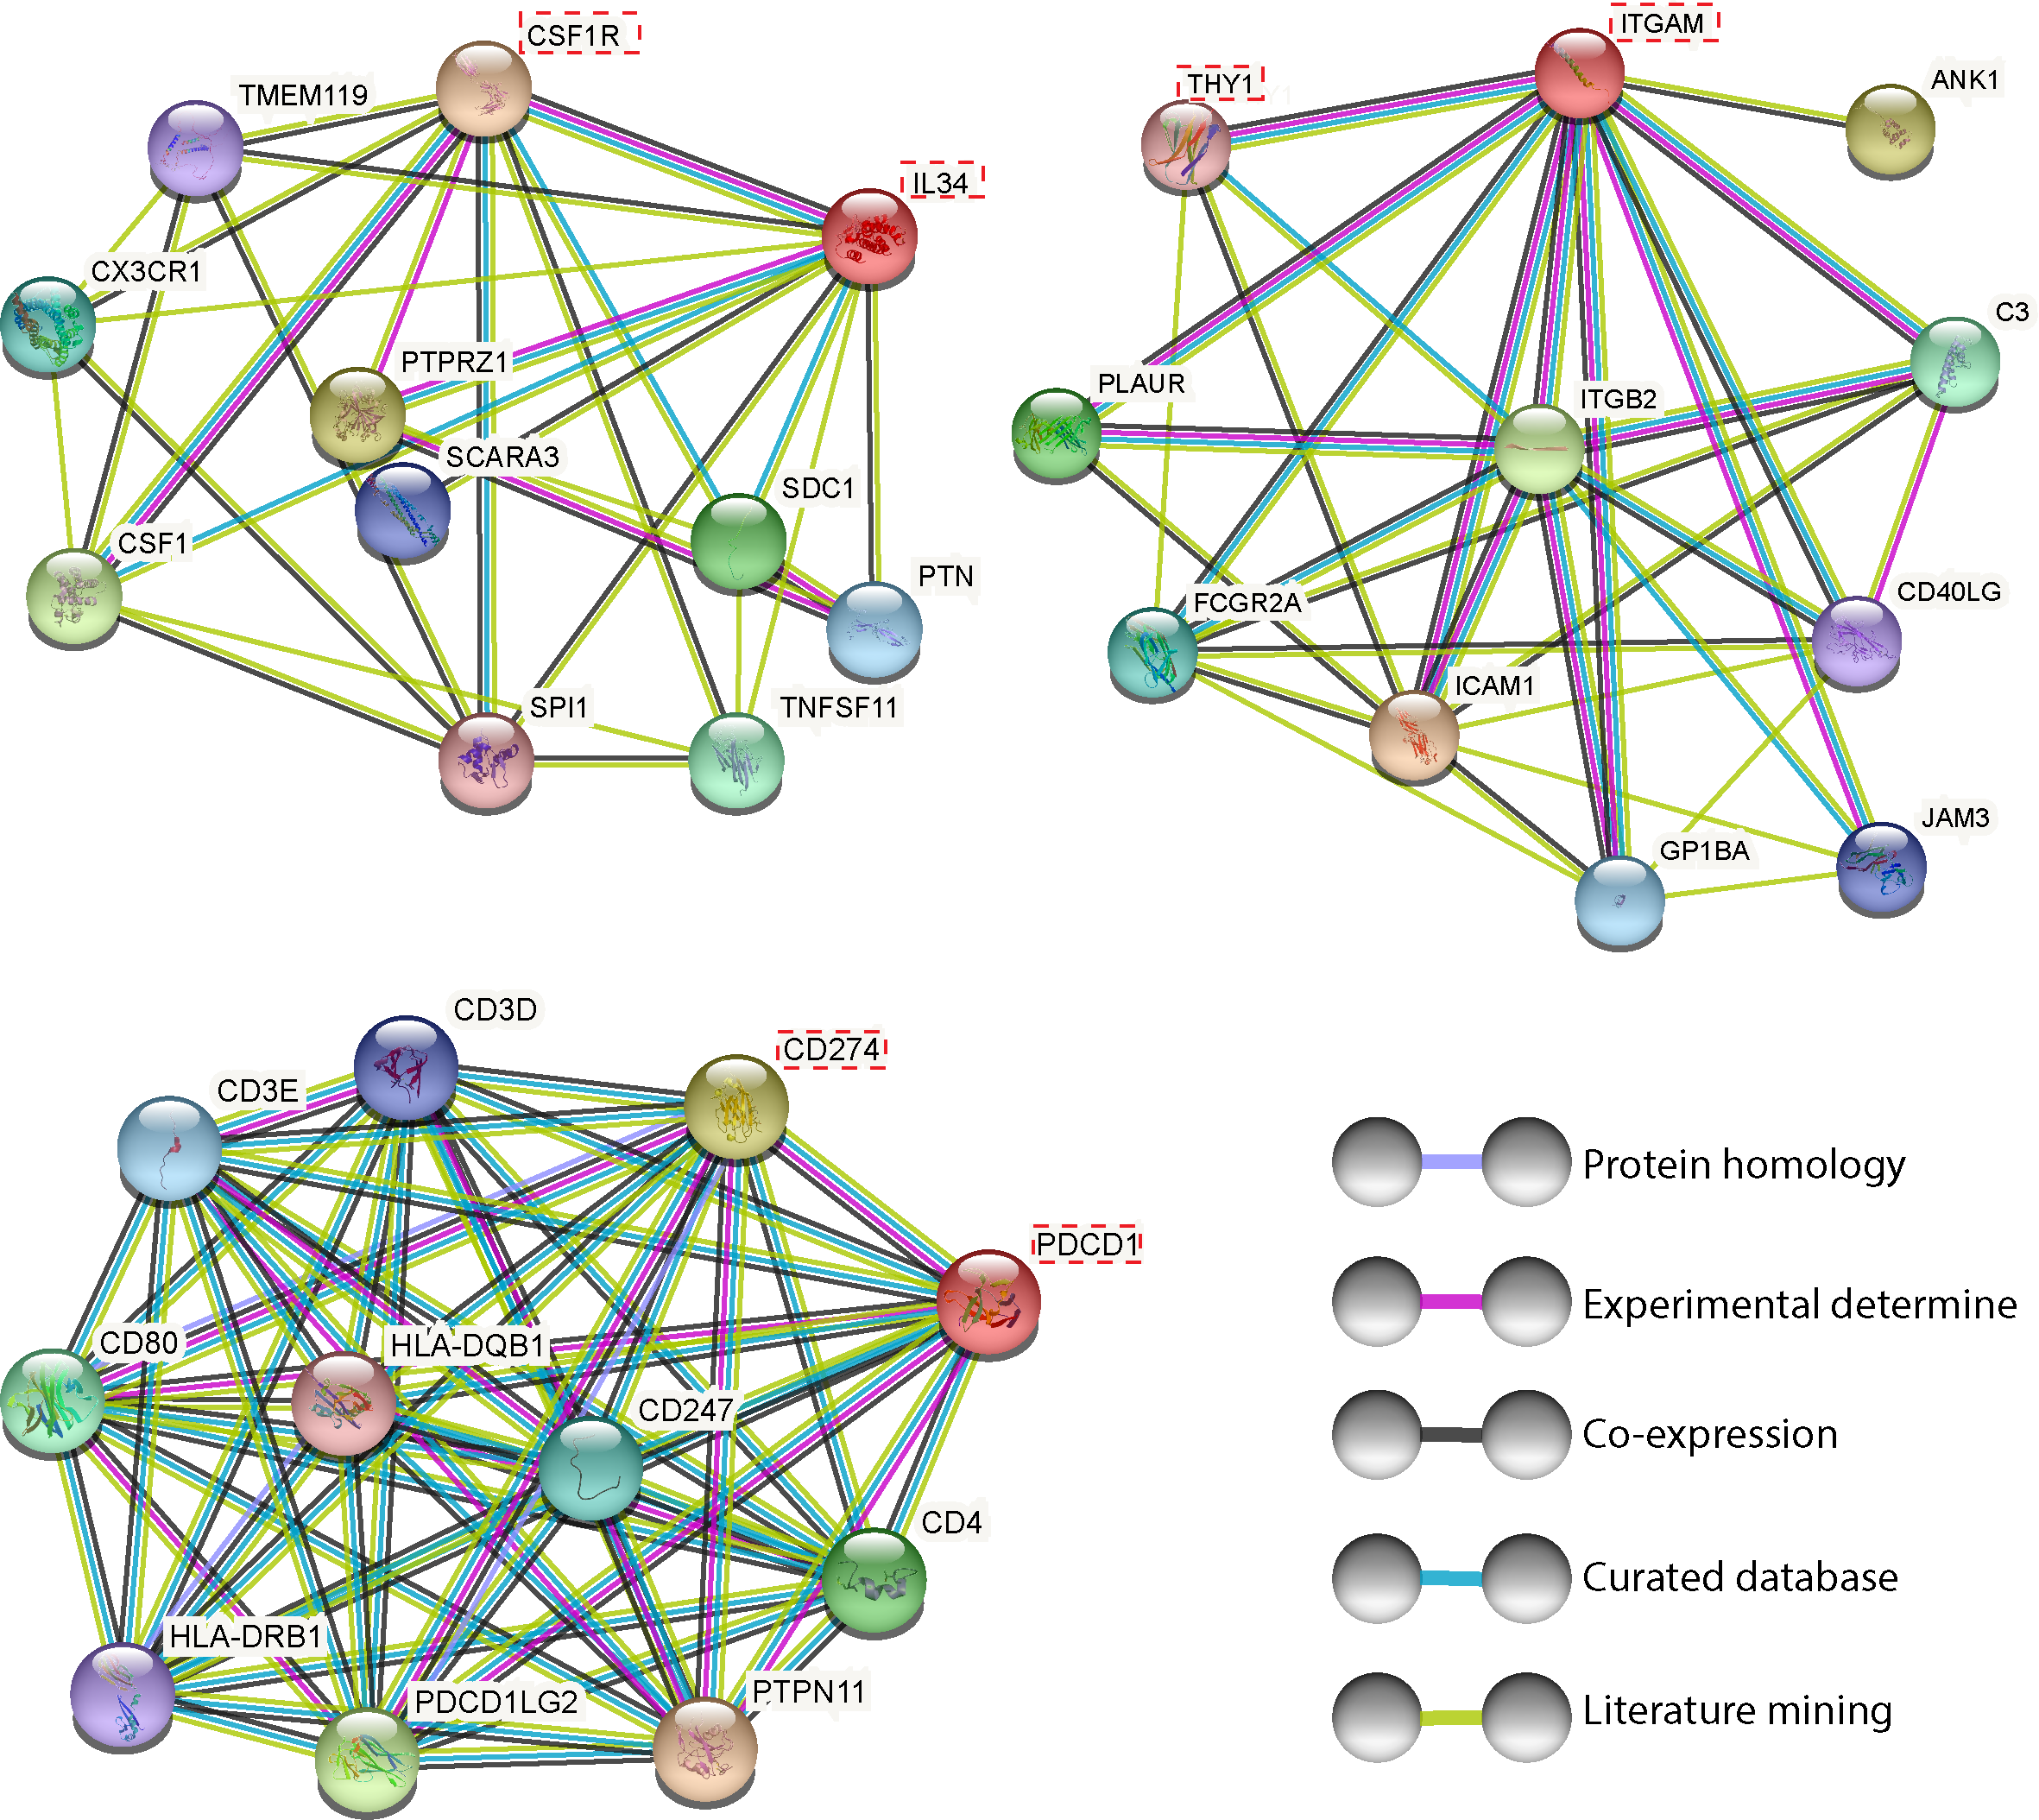
\includegraphics[width=0.66\columnwidth]{Chapter2/Figures/Supplemental_Fig_S1.png}
    \caption{Interaction networks of the 3 ligand-receptor pairs namely, CSF1R-IL34, ITGAM-THY1 and PD1-PD-L1. Each node represents a protein and is connected to each other by multple edges which indicate the possibility of interaction between each pair. The edges are colored by the method which was used to determine the interaction}
    \label{fig:Chap2_Supfigure1}
\end{figure}
\begin{figure}[htp]
    \centering
    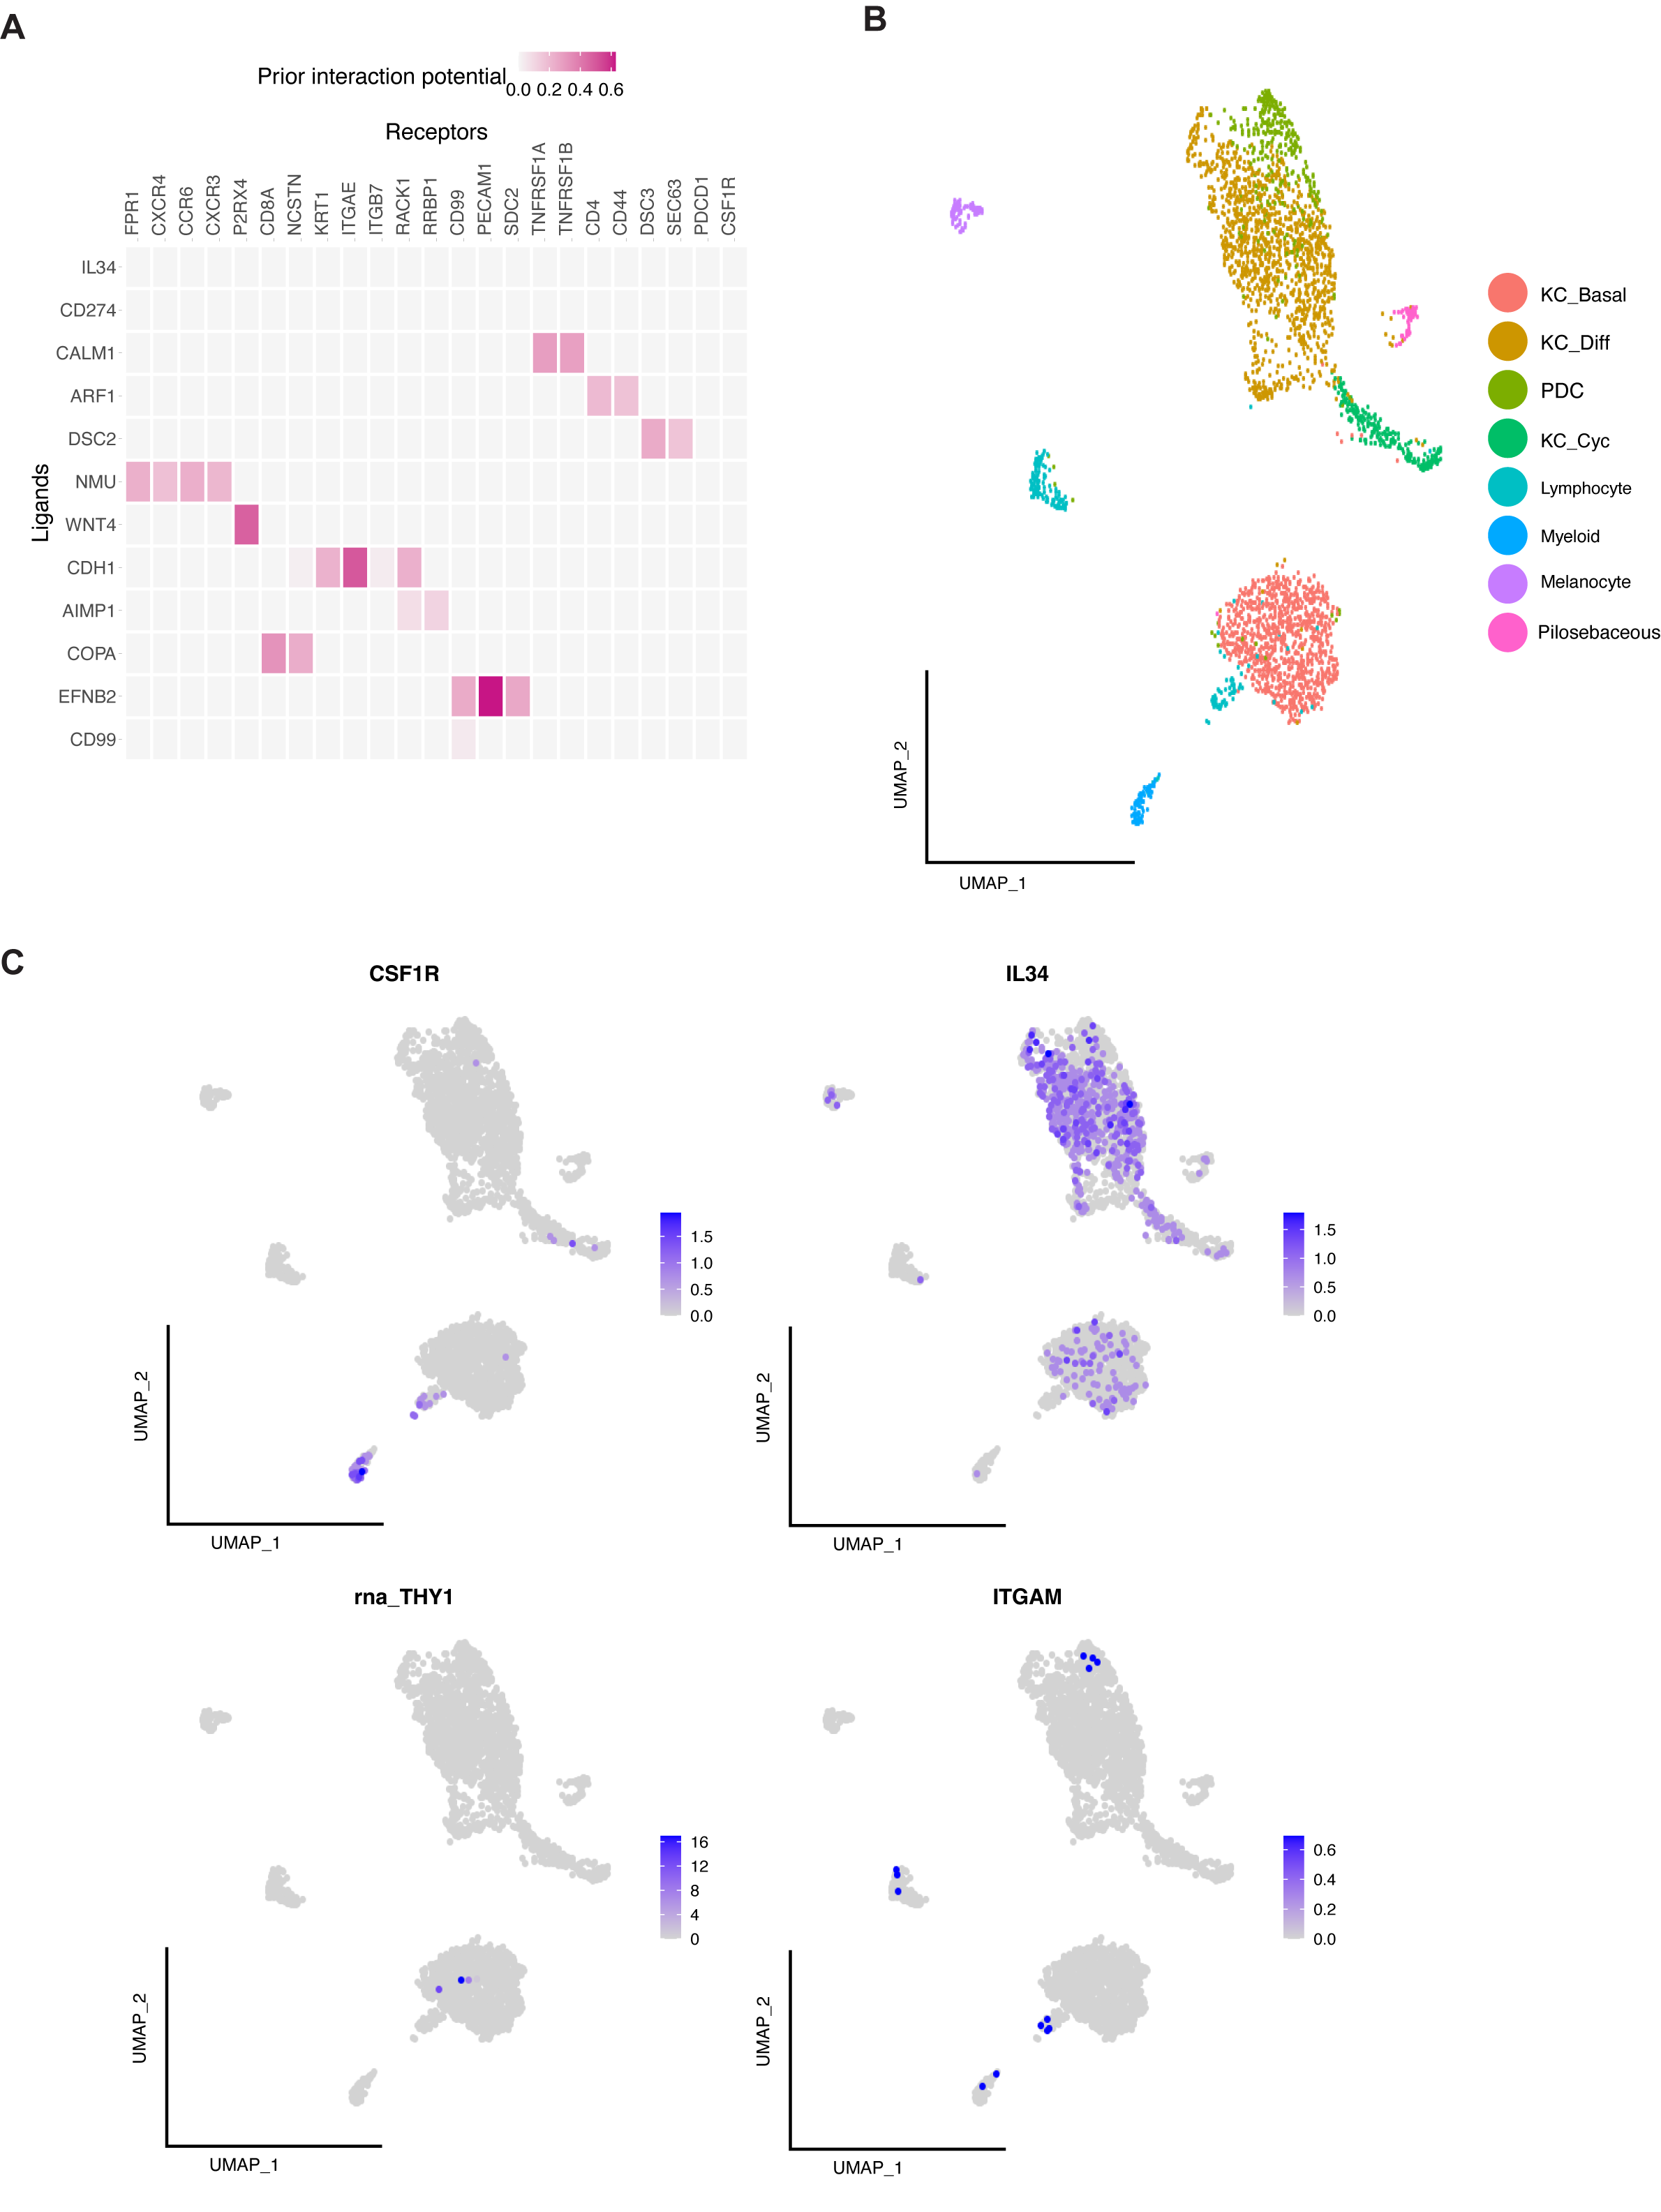
\includegraphics[width=0.75\columnwidth]{Chapter2/Figures/Supplemental_Fig_S2.png}
    \caption{scRNA-seq ligand-receptor interaction analysis of SCC cancer patient sample. (A) NicheNet analysis results, with a heatmap showing ligand-receptor predicted interaction potential for the top 12 ligands. (B) A UMAP plot with cells grouped into 14 clusters using Louvain algorithm and gene expression. Each cluster is shown as one color. One dot represents a cell. (C) A feature plot highlighting (navy dots) the distribution of cells expressing IL34 (left plot) and CSF1R (right plot). (D) A feature plot highlighting the distribution of cells expressing THY1 and ITGAM. Cells without expression appear as grey dots.}
    \label{fig:Chap2_Supfigure2}
\end{figure}
\begin{figure}[htp]
\renewcommand{\figurename}{Supplementary Figure}
    \centering
    \includegraphics[width=0.75\columnwidth]{Chapter2/Figures/Supplemental_Fig_S3.png}
    \caption{ST-seq expression and cell-type analysis of the BCC skin cancer Visium data. (A) A QC plot showing the number of genes and reads captured in each spot across the whole BCC tissue section. (B) The number of transcripts captured in each spot after stLearn normalization. stLearn imputed the signals of lowly expressed genes, using tissue morphological correlation (Pham et al, 2020). (C) The gene expression levels of IL34 and CSF1R (before normalization) displayed across all spots across the tissue. (D) A spatial feature plot of the gene expression levels of ITGAM and THY1. (E) The stlearn’s statistic visualization of significant spots using the pair of ligand-receptor IL34 and CSF1R (the color bar shows the -log10 of the p-values)}
    \label{fig:Chap2_Supfigure3}
\end{figure}
\begin{figure}[htp]
\renewcommand{\figurename}{Supplementary Figure}
    \centering
    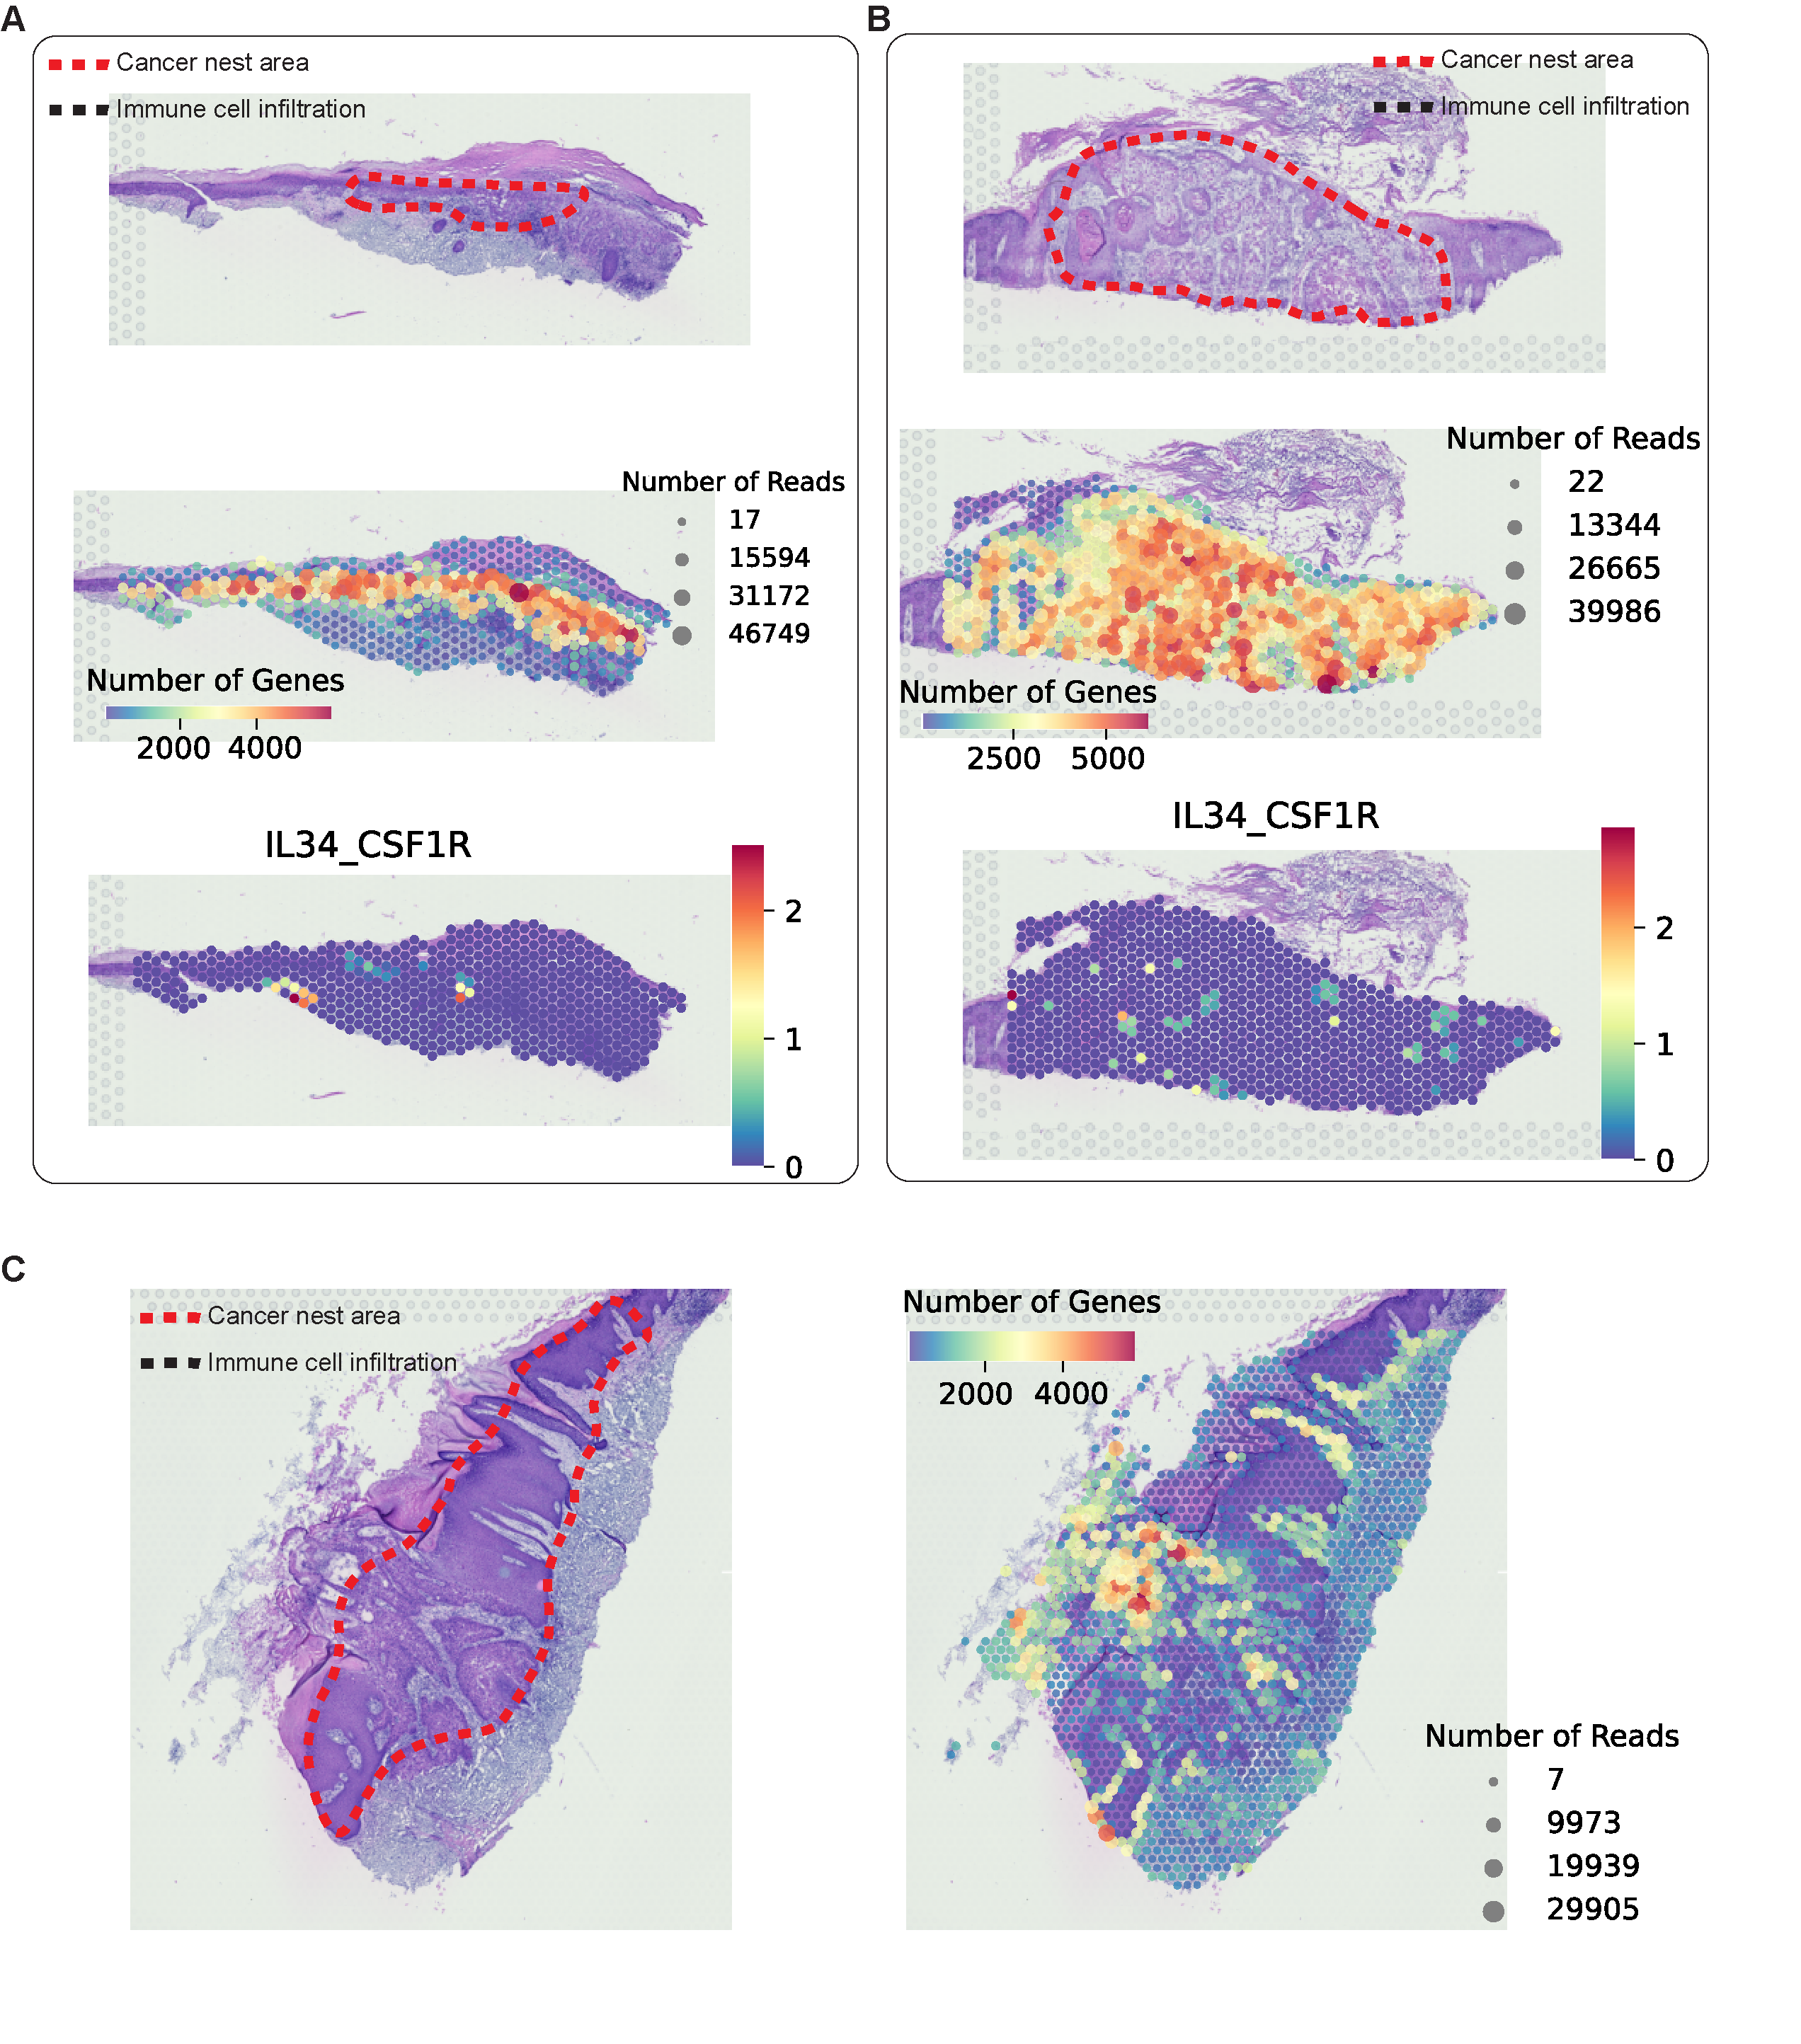
\includegraphics[width=0.75\columnwidth]{Chapter2/Figures/Supplemental_Fig_S4.png}
    \caption{Visium spatial transcriptomic for infering cell interaction through ligand-receptor and interaction sites with spatial contexts (related to Supplemental Table 1). (A) From top to bottom, a H\&E image, the ST-seq captured and the significant spots of interaction using the pair of L-R IL34 and CSF1R (the color bar shows the -log10 of the p-values) of BCC tissue section of patient ID-B18. (B) the H\&E image (top), the ST-seq profile of SCC patient ID-E15(middle) and the corresponding spatial distribution of significant spot with cell interaction through the pair of L-R IL34-CSF1R (bottom). (C) the H\&E image and the ST-seq captured from SCC patient ID-F21. }
    \label{fig:Chap2_Supfigure4}
\end{figure}
\begin{figure}[htp]
\renewcommand{\figurename}{Supplementary Figure}
    \centering
    \includegraphics[width=0.75\columnwidth]{Chapter2/Figures/Supplemental_Fig_S5.png}
    \caption{RNAscope scanning images from different tissue samples (related to Supplemental Table 1). (A) Whole tissue scanning and STRISH analysis results on the tissue sample from BCC patient ID-B18. From bottom left to right, the heatmaps of significant windows of locals co-expression for two L-R pairs, IL34-CSF1R and ITGAM-THY1 respectively. Similarly (B) shows the whole tissue scanning and STRISH analysis results of SCC patient ID-D04 with the target L-R pairs are IL34-CSF1R and ITGAM-THY1. (C) and (D) are the whole slide flourescent images captured by the RNAscope in two SCC tissues from patients ID-F21 and ID-E15 respectively. Pseudo-coloring are applied to RNAscope flourescene probe following the color legend.}
    \label{fig:Chap2_Supfigure5}
\end{figure}
\begin{figure}[htp]
\renewcommand{\figurename}{Supplementary Figure}
    \centering
    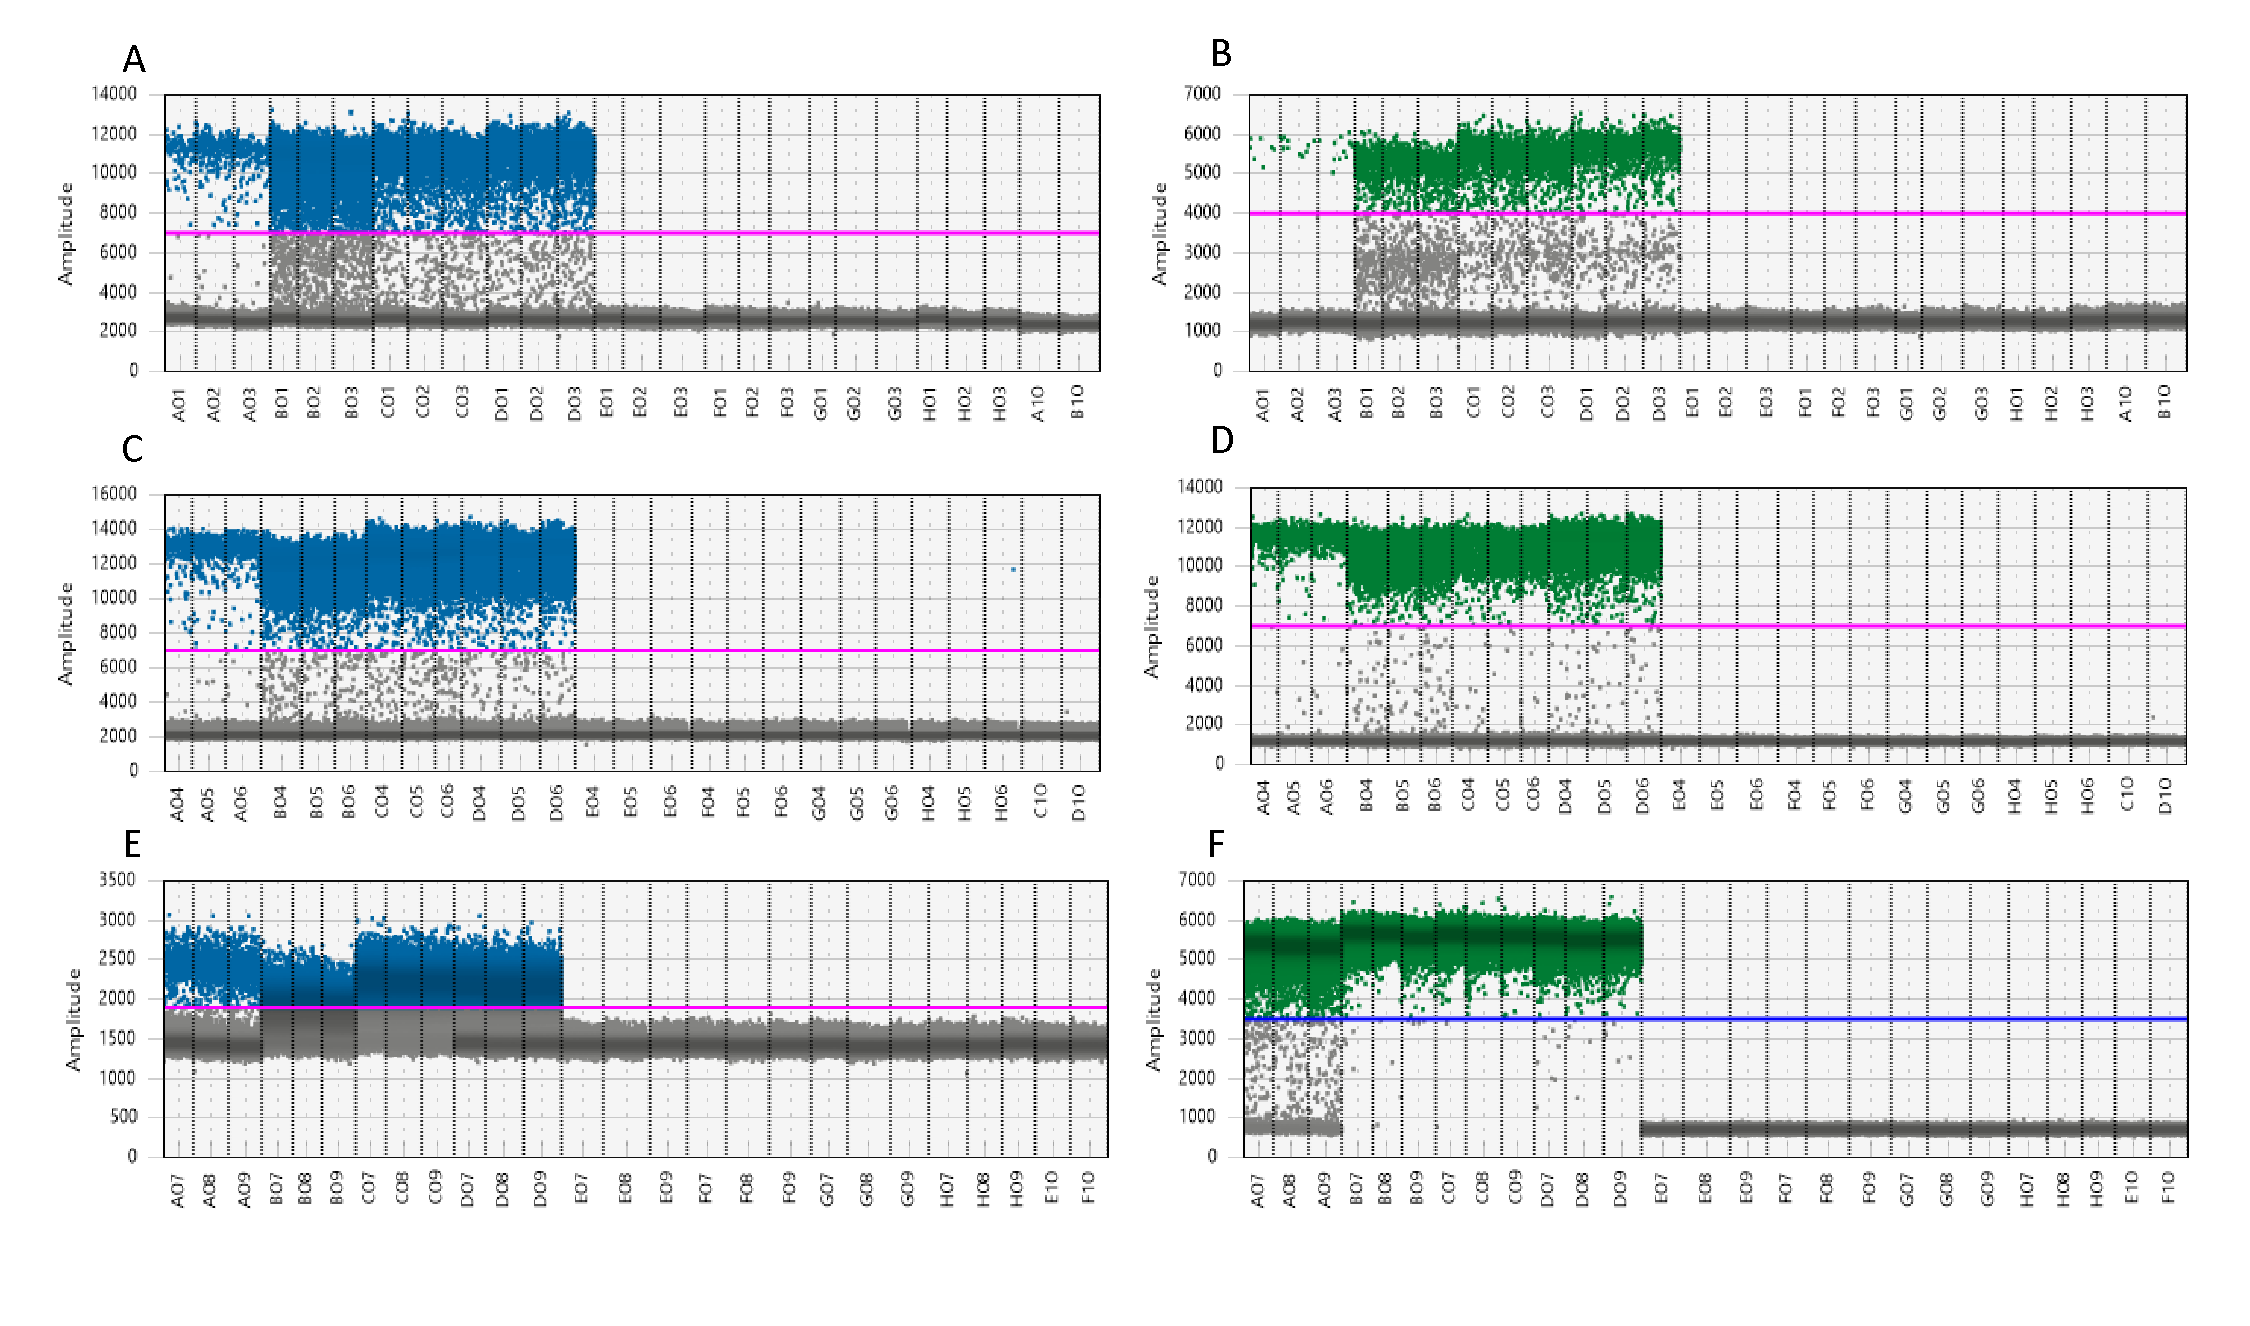
\includegraphics[width=0.75\columnwidth]{Chapter2/Figures/Supplemental_Fig_S6.png}
    \caption{Analysis of target genes by automated droplet digital PCR. Expression plots for data from the three BCC patients and negative controls are shown. Each blue or green point represents a single droplet. The negative droplets scored as grey if the fluorescent amplitude is lower than a detection threshold. The solid pink line indicates the threshold. FAM and HEX are reporter fluorophores conjugated to ddPCR primers to amplify templates that were later read by the QX200 droplet reader. Each gene in each droplet was read based on the labeled primer, specific for the gene.  }
    \label{fig:Chap2_Supfigure6}
\end{figure}
\begin{figure}[htp]
\renewcommand{\figurename}{Supplementary Figure}
    \centering
    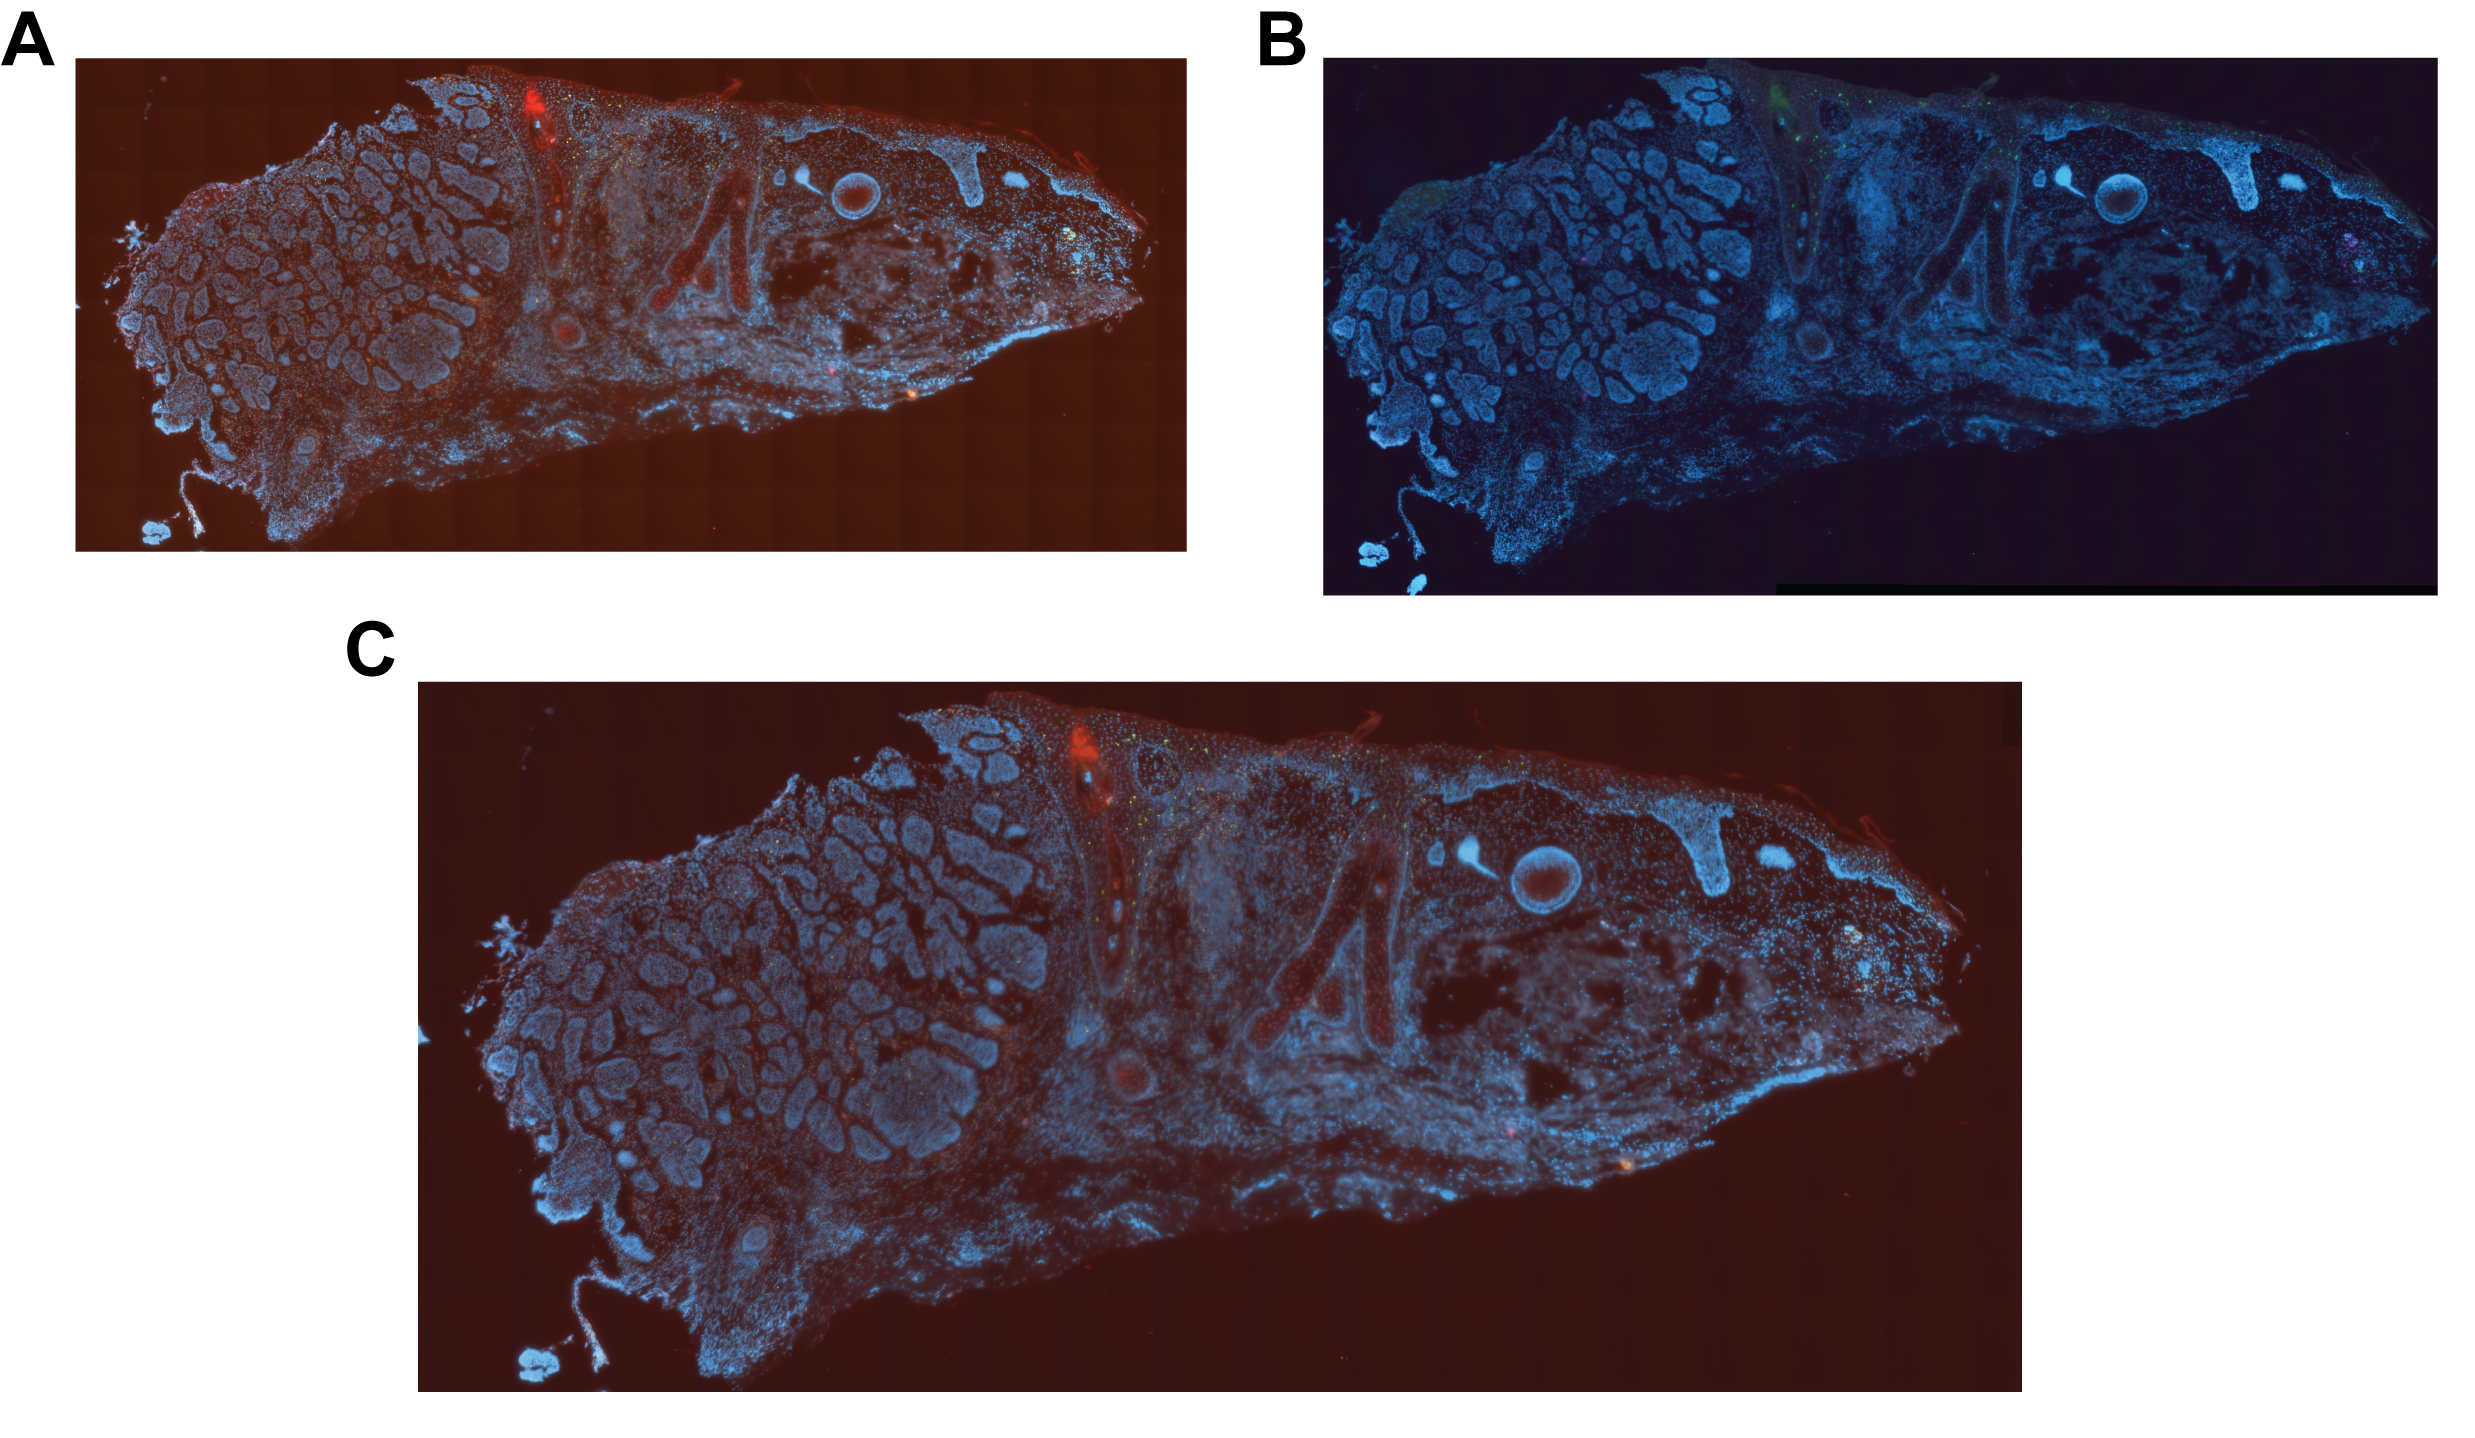
\includegraphics[width=0.75\columnwidth]{Chapter2/Figures/Supplemental_Fig_S7.png}
    \caption{Outputs from two steps in the STRISH analysis pipeline for RNAscope images registration. (A) The RNAscope image for THY1, IL34, and CSF1R signals from the first round of imaging. (B) The RNAscope image for ITGAM and CD207 signals from the second round of imaging (for the same tissue section). (C) The result of image registration to combine the outputs from the two imaging rounds. After registration, the results from the two hybridization rounds (\ie THY1 and ITGAM) were compatible with the local co-expression analysis.}
    \label{fig:Chap2_Supfigure7}
\end{figure}
\typeout{}

% \bibliographystyle{elsarticle-num}

% \bibliography{./References/Bibliography}